\section{Rank 2 theories}\label{sec:rank2 theories}

In this section, we will compute the BPS spectra of all rank-2 KK theories by employing our bootstrap approach. The computations will then guarantee that all rank-2 5d and 6d QFTs have solvable blowup equations and their BPS spectra can be obtained by the bootstrap method. To support our claim, we will present computations of the BPS spectra of three non-geometric 5d SCFTs: $SU(3)_8$, $\mathbb{P}^2 \cup \mathbb{F}_3+1{\bf Sym}$, and $\mathbb{P}^2 \cup \mathbb{F}_6+1{\bf Sym}$.


\subsection{KK theories}
In this subsection, we solve the blowup equations for all rank-2 5d KK theories classified in \cite{Jefferson:2017ahm,Jefferson:2018irk,Bhardwaj:2019fzv}.


\subsubsection{\texorpdfstring{$Sp(2)+3\mathbf{\Lambda}^2$}{Sp(2) + 3AS}}
 
The 5d $ Sp(2)$ gauge theory with 3 anti-symmetric hypermultiplets ($Sp(2)+3\mathbf{\Lambda}^2$) is the KK-theory arising from the twisted compactification of the 6d $ SU(3) $ gauge theory with 6 fundamental hypermultiplets,
\begin{align}
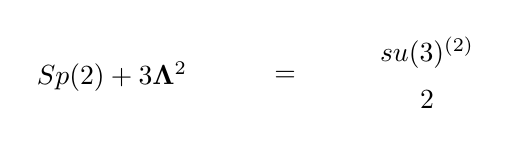
\begin{tikzpicture}
\draw (0, 0) node {$ Sp(2) + 3\mathbf{\Lambda}^2 $}
(2.2, 0) node {$ = $}
(4, 0.3) node {$ \mathfrak{su}(3)^{(2)} $}
(4, -0.3) node {$ 2 $};
\end{tikzpicture}
\end{align}
This theory has a geometric description \cite{Jefferson:2018irk} as 
\begin{align}\label{eq:Sp2_3AS_geo}
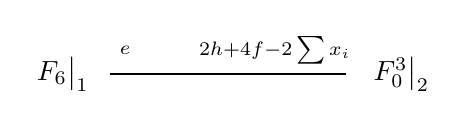
\begin{tikzpicture}
\draw[thick](-3,0)--(0,0);	
\node at(-3.6,0) {$\mathbb{F}_{6}{}\big|_1$};
\node at(-2.8,0.3) {${}_e$};
\node at(0.7,0) {$\mathbb{F}_{0}^{3}{}\big|_2$};
\node at(-0.9,0.3) {${}_{2h + 4f - 2\sum x_i}$};
\end{tikzpicture}
\end{align}
and the fiber-base duality of $\mathbb{F}_0^3$ exchanges two dual descriptions: the 5d $Sp(2)$ gauge theory with 3 anti-symmetric hypers and the 6d $SU(3)$ gauge theory with 6 fundamentals on a circle with $\mathbb{Z}_2$ twist.

In 5d $Sp(2)$ gauge theory description, the cubic prepotential on the chamber described by the above geometry
 is
\begin{align}
6\mathcal{F}
&= 8\phi_1^3 + 12\phi_1^2 \phi_2 - 18\phi_1 \phi_2^2 + 8\phi_2^3 + 6m_0 (2\phi_1^2 - 2\phi_1 \phi_2 + \phi_2^2) \\
& \quad - \frac{1}{2} \sum_{i=1}^3 \qty((\phi_2 + m_i)^3 + (2\phi_1 - \phi_2 + m_i)^3 + (-2\phi_1 + \phi_2 + m_i)^3 + (\phi_2 - m_i)^3) \, , \nonumber
\end{align}
where $ m_0 $ is the gauge coupling and $ m_{i=1, 2, 3} $ are mass parameters for the 3 antisymmetric hypermultiplets. The full effective prepotential on the $\Omega$-background is
\begin{align}
\mathcal{E}
= \frac{1}{\epsilon_1 \epsilon_2} \left(\mathcal{F} - \frac{\epsilon_1^2 + \epsilon_2^2}{48} (4\phi_1 - 2\phi_2) + \epsilon_+^2 (\phi_1 + \phi_2) \right) \, .
\end{align}

The volumes of the primitive 2-cycles in the geometry \eqref{eq:Sp2_3AS_geo} in terms of the $Sp(2)$ gauge theory parameters can be written as
\begin{align}
&\vol (f_1) = 2\phi_1 - \phi_2 \, , \quad
&&\vol (f_2) = -2\phi_1 + 2\phi_2 \, , \nonumber \\
&\vol (e_2) = -4\phi_1 + 2\phi_2 + m_0 \, , \quad
&&\vol (x_i) = -2\phi_1 + \phi_2 + m_i \quad (i = 1, 2, 3) \, .
\end{align}
From this information, we can choose a set of magnetic fluxes as
\begin{align}
n_i \in \mathbb{Z} \, , \quad
B_{m_0} = 0 \, , \quad
B_{m_i} = 1/2 \quad (i = 1, 2, 3) \, ,
\end{align}
which gives rise to a unity blowup equation. The unity blowup equation can be easily solved and the resulting BPS spectrum is summarized in Table~\ref{table:Sp2_3AS}.

\begin{table}
	\centering
	\begin{tabular}{|c|C{25ex}||c|C{25ex}|} \hline
		$ \mathbf{d} $ & $ \oplus N_{j_l, j_r}^{\mathbf{d}} (j_l, j_r) $ & $ \mathbf{d} $ & $ \oplus N_{j_l, j_r}^{\mathbf{d}} (j_l, j_r) $ \\ \hline
		$ (1, 0, 0, -1) $ & $ 3(0, 0) $ & $ (1, 0, 0, 0) $ & $ (0, \frac{1}{2}) $ \\ \hline
		$ (1, 0, 1, -3) $ & $ (0, 0) $ & $ (1, 0, 1, -2) $ & $ 3(0, \frac{1}{2}) $ \\ \hline
		$ (1, 0, 1, -1) $ & $ 3(0, 1) $ & $ (1, 0, 1, 0) $ & $ (0, \frac{3}{2}) $ \\ \hline
		$ (1, 1, 0, 0) $ & $ (0, \frac{1}{2}) $ & $ (1, 1, 1, -2) $ & $ 3(0, \frac{1}{2}) $ \\ \hline
		$ (1, 1, 1, -1) $ & $ 3(0, 0) \oplus 3(0, 1) $ & $ (1, 1, 1, 0) $ & $ (0, \frac{1}{2}) \oplus (0, \frac{3}{2}) $ \\ \hline
		$ (2, 0, 1, -3) $ & $ (0, 1) $ & $ (2, 0, 1, -2) $ & $ 3(0, \frac{3}{2}) $ \\ \hline
		$ (2, 0, 1, -1) $ & $ 3(0, 2) $ & $ (2, 0, 1, 0) $ & $ (0, \frac{5}{2}) $ \\ \hline
		$ (2, 1, 1, -3) $ & $ (0, 0) \oplus (0, 1) $ & $ (2, 1, 1, -2) $ & $ 3(0, \frac{1}{2}) \oplus 3(0, \frac{3}{2}) $ \\ \hline
		$ (2, 1, 1, -1) $ & $ 3(0, 1) \oplus 3(0, 2) $ & $ (2, 1, 1, 0) $ & $ (0, \frac{3}{2}) \oplus (0, \frac{5}{2}) $ \\ \hline
	\end{tabular}
	\caption{BPS spectrum of $ Sp(2) + 3\mathbf{\Lambda}^2 $ for $ d_1 \leq 2 $, $ d_2 \leq 1 $, $ d_3 \leq 1 $. Here, $ \mathbf{d} = (d_1, d_2, d_3, d_4) $ labels the BPS states with charge $ d_1 e_2 + d_2 f_1 + d_3 f_2 + d_4 x_i $ and $d_4$ counts collective degrees of all anti-symmetric hypermultiplets.} \label{table:Sp2_3AS}
\end{table}

Now we consider the 6d $SU(3)$ gauge theory. Under the $\mathbb{Z}_2$ twist, the vector multiplet and the hypermultiplets in 6d are decomposed into the representations of the invariant subalgebra $\mathfrak{su}(2)$ as
\begin{align}
\mathbf{8} \text{ of } \mathfrak{su}(3) \ &\to \ \mathbf{3}_0 \oplus \mathbf{2}_{1/4} \oplus \mathbf{2}_{3/4} \oplus \mathbf{1}_{1/2} \text{ of } \mathfrak{su}(2)\ , \nonumber \\
\mathbf{3} \oplus \bar{\mathbf{3}} \text{ of } \mathfrak{su}(3) \ &\to \ \mathbf{2}_0 \oplus \mathbf{1}_{1/4} \oplus \mathbf{2}_{1/2} \oplus \mathbf{1}_{3/2} \text{ of } \mathfrak{su}(2) \ ,
\end{align}
where the subscripts denote the shifted KK charges due to the $\mathbb{Z}_2$ twist. Collecting the 1-loop contributions from these KK states and the classical Green-Schwarz contributions, we obtain the full effective prepotential on the $\Omega$-background as
\begin{align}
\mathcal{E} \label{eq:su3_2_E}
&=\frac{1}{\epsilon_1 \epsilon_2} \bigg( \mathcal{E}_{\mathrm{tree}} + \mathcal{F}_{\text{1-loop}} + \frac{\epsilon_1^2 + \epsilon_2^2}{24}\phi_1 + \epsilon_+^2 \phi_1 \bigg) \ , \nonumber \\
\mathcal{E}_{\mathrm{tree}}
&= \tau \phi_0^2 + 2\phi_0 \qty( \phi_1^2 - \frac{1}{2}\sum_{i=1}^3 m_i^2 + \frac{3}{2} \epsilon_+^2 )\ , \nonumber  \\
%
\mathcal{F}_{\text{1-loop}}
&= \frac{5}{6}\phi_1^3 - \frac{3}{16}\tau \phi_1^2 - \frac{1}{2} \sum_{i=1}^3 m_i^2 \phi_1\ . 
\end{align}
Here, the K\"ahler parameters in the 6d gauge theory description can be converted to the parameters in the 5d $Sp(2)$ gauge theory description simply by the following reparametrization:
\begin{align}
&\phi_0 \to \phi_1 + \frac{m_0}{16} - \frac{1}{4} \sum_{i=1}^3 m_i\,, \quad
\phi_1 \to \phi_2 - 2\phi_1 + \frac{m_0}{2}\,, \quad
\tau \to 2m_0\,,  \quad
m_i \to m_i - \frac{m_0}{2} \,.
\end{align}
One can easily check that the effective prepotential of the 6d theory with this reparametrization reproduces that of the 5d theory given above up to terms independent of $\phi_i$.

It is convenient in the 6d perspective to use the 6d parameters shifted as
\begin{align}
\phi_0 \to \phi_0 - \frac{5}{32}\tau - \frac{1}{4}\sum_{i=1}^3 m_i\, , \quad
\phi_1 \to \phi_1 - 2\phi_0 \, .
\end{align}
The volumes of 2-cycles in the geometry \eqref{eq:Sp2_3AS_geo} can be written in terms of the shifted 6d parameters as
\begin{align}
&\vol (f_1) = 2\phi_0 - \phi_1 + \frac{\tau}{4}\,, \quad
&&\vol (f_2) = -4\phi_0 + 2\phi_1\,, \nonumber \\
&\vol (e_2) = -2\phi_0 + 2\phi_1 - \frac{\tau}{2}\,, \quad
&&\vol (x_i) = -2\phi_0 + \phi_1 + m_i \, .
\end{align}
One finds a pair of consistent magnetic fluxes as
\begin{align}
	n_1 \in \mathbb{Z} \, , \quad B_\tau = 0 \,, \quad B_{m_i}=1/2 \,, \quad n_0\in \mathbb{Z}+B_{0} \quad {\rm with} \quad B_0 = 0,1/2  \, ,
\end{align}
which lead to unity blowup equations. We checked that the solutions to the blowup equations match the result in Table~\ref{table:Sp2_3AS} from the 5d $Sp(2)$ gauge theory.


\subsubsection{\texorpdfstring{$SU(3)_4+6\mathbf{F}$, $Sp(2)+2\mathbf{\Lambda}^2+4\mathbf{F}$, $G_2+6\mathbf{F}$}{SU(3)4 + 6F}}

This theory is a KK theory coming from the 6d $ SU(3)$ gauge theory with 12 fundamental hypermultiplets on a circle with $ \mathbb{Z}_2 $ twist. It has three different 5d gauge theory descriptions: $ SU(3)_4 + 6\mathbf{F} $, $ Sp(2) + 2\mathbf{\Lambda}^2 + 4\mathbf{F} $, and  $G_2+6\mathbf{F}$,
\begin{align}
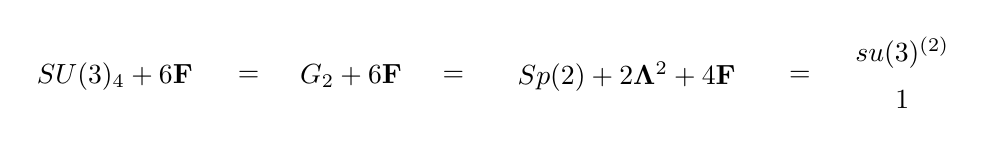
\begin{tikzpicture}
\draw (0, 0) node {$ SU(3)_4 + 6\mathbf{F} $}
(1.7, 0) node {$ = $}
(3, 0) node {$ G_2 + 6\mathbf{F} $}
(4.3, 0) node {$ = $}
(6.5, 0) node {$ Sp(2) + 2\mathbf{\Lambda}^2 + 4\mathbf{F} $}
(8.7, 0) node {$ = $}
(10, 0.3) node {$ \mathfrak{su}(3)^{(2)} $}
(10, -0.3) node {$ 1 $};
\end{tikzpicture}
\end{align}
This theory is geometrically engineered by gluing $ \mathbb{F}_2 $ and $ \mathbb{F}_0^6 $ as \cite{Jefferson:2018irk}
\begin{align}
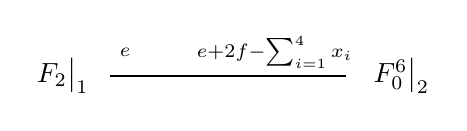
\begin{tikzpicture}
\draw[thick](-3,0)--(0,0);	
\node at(-3.6,0) {$\mathbb{F}_{2}{}\big|_1$};
\node at(-2.8,0.3) {${}_e$};
\node at(0.7,0) {$\mathbb{F}_{0}^{6}{}\big|_2$};
\node at(-0.9,0.3) {${}_{e + 2f - \sum_{i=1}^4 x_i}$};
\end{tikzpicture}
\end{align}

We shall solve the blowup equations by using the $ SU(3) $ and $ G_2 $ frames. We first compute the cubic prepotential of the $SU(3)$ gauge theory on the chamber $\phi_2\ge \phi_1>0$ as
\begin{align}
6\mathcal{F}
&= 8\phi_1^3 - 3\phi_1^2 \phi_2 - 3\phi_1 \phi_2^2 + 8\phi_2^2 + 12\phi_1 \phi_2(\phi_1 - \phi_2) \\
& \quad - \frac{1}{2} \sum_{i=1}^6 \Big((\phi_2 - m_i)^3 + (\phi_2 - \phi_1 + m_i)^3 + (\phi_1 + m_i)^3\Big) + 6m_0(\phi_1^2 - \phi_1 \phi_2 + \phi_2^2) \, ,  \nonumber
\end{align}
where $ m_0 $ is the $ SU(3) $ gauge coupling and $ m_{i=1, \cdots, 6} $ are mass parameters of 6 fundamentals. The full effective prepotential is
\begin{align}
\mathcal{E}
= \frac{1}{\epsilon_1 \epsilon_2} \qty(\mathcal{F} - \frac{\epsilon_1^2 + \epsilon_2^2}{48}(4\phi_1 - 8\phi_2 ) + \epsilon_+^2 (\phi_1 + \phi_2) ) \, .
\end{align}
A choice of magnetic fluxes
\begin{align}
n_i \in \mathbb{Z} \, , \quad
B_{m_0} = -1/2 \, , \quad
B_{m_i} = 1/2 \quad (1 \leq i \leq 6) \, 
\end{align}
provides a solvable unity blowup equation. We solve the blowup equation and find the BPS spectrum of the $SU(3)_4+6{\bf F}$ theory listed in Table~\ref{table:SU3_4_6F}.
\begin{table}
	\centering
	\begin{tabular}{|c|C{25ex}||c|C{25ex}|} \hline
		$ \mathbf{d} $ & $ \oplus N_{j_l, j_r}^{\mathbf{d}} (j_l, j_r) $ & $ \mathbf{d} $ & $ \oplus N_{j_l, j_r}^{\mathbf{d}} (j_l, j_r) $ \\ \hline
		$ (1, -\frac{4}{3}, \frac{1}{3}) $ & $ (0, \frac{1}{2}) $ & $ (1, -\frac{4}{3}, \frac{4}{3}) $ & $ (0, \frac{3}{2}) $ \\ \hline
		$ (1, -1, 0) $ & $ 6(0, 0) $ & $ (1, -1, 1) $ & $ 6(0, 1) $ \\ \hline
		$ (1, -1, 2) $ & $ 6(0, 2) $ & $ (1, -\frac{2}{3}, \frac{2}{3}) $ & $ 15(0, \frac{1}{2}) $ \\ \hline
		$ (1, -\frac{2}{3}, \frac{5}{3}) $ & $ 15(0, \frac{3}{2}) $ & $ (1, -\frac{1}{3}, \frac{1}{3}) $ & $ 20(0, 0) \oplus (0, \frac{1}{2}) $ \\ \hline
		$ (1, -\frac{1}{3}, \frac{4}{3}) $ & $ (0,\frac{1}{2}) \oplus 20(0,1) \oplus (0,\frac{3}{2}) $ & $ (1, 0, 1) $ & $ 6(0,0) \oplus 15(0,\frac{1}{2}) \oplus 6(0,1) $ \\ \hline
		$ (1, 0, 2) $ & $ 6(0,1) \oplus 15(0,\frac{3}{2}) \oplus 6(0,2) $ & $ (1, \frac{1}{3}, \frac{2}{3}) $ & $ 6(0,0) \oplus 15(0,\frac{1}{2}) $ \\ \hline
		$ (1, \frac{1}{3}, \frac{5}{3}) $ & $ \! 15(0,\frac{1}{2}) \oplus 6(0,1) \oplus 15(0,\frac{3}{2}) \! $ & $ (1, \frac{2}{3}, \frac{1}{3}) $ & $ 20(0,0) \oplus (0,\frac{1}{2}) $ \\ \hline
		$ (1, \frac{2}{3}, \frac{4}{3}) $ & $ 20(0,0) \oplus 2(0,\frac{1}{2}) \oplus 20(0,1) \oplus (0,\frac{3}{2}) $ & $ (1, 1, 0) $ & $ 6(0, 0) $ \\ \hline
		$ (1, 1, 1) $ & $ 6(0,0) \oplus 15(0,\frac{1}{2}) \oplus 6(0,1) $ & $ (1, 1, 2) $ & $ 6(0,0) \oplus 15(0,\frac{1}{2}) \oplus 6(0,1) \oplus 15(0,\frac{3}{2}) \oplus 6(0,2) $ \\ \hline
		$ (2, -2, 1) $ & $ 15(0, \frac{3}{2}) $ & $ (2, -\frac{5}{3}, \frac{2}{3}) $ & $ 20(0, 1) $  \\ \hline
		$ (2, -\frac{4}{3}, \frac{1}{3}) $ & $ 15(0, \frac{1}{2}) $ & $ (2, -1, 0) $ & $ 6(0, 0) $ \\ \hline
		$ (2, -1, 1) $ & $ 6(0,0) \oplus 15(0,\frac{1}{2}) \oplus 96(0,1) \oplus 15(0,\frac{3}{2}) \oplus 6(\frac{1}{2},\frac{3}{2}) $ & $ (2, -\frac{2}{3}, \frac{2}{3}) $ & $ 20(0,0) \oplus 37(0,\frac{1}{2}) \oplus 20(0,1) \oplus	(\frac{1}{2},1) $  \\ \hline
		$ (2, -\frac{1}{3}, \frac{1}{3}) $ & $ 12(0,0) \oplus 15(0,\frac{1}{2}) $ & $ (2, 0, 1) $ & $ 102(0,0) \oplus 66(0,\frac{1}{2}) \oplus 102(0,1) \oplus 15(0,\frac{3}{2}) \oplus 6(\frac{1}{2},\frac{1}{2}) \oplus 6(\frac{1}{2},\frac{3}{2}) $  \\ \hline
	\end{tabular}
	\caption{BPS spectrum of the $ SU(3)_4 + 6\mathbf{F} $ theory for $ (d_1 = 1, d_2 \leq 1, d_3 \leq 2) $ and $ (d_1 = 2, d_2 \leq 0, d_3 \leq 1) $ where $ \mathbf{d} = (d_1, d_2, d_3) $ labels the BPS states with charge $ d_1 m_0 + d_2 \alpha_1 + d_3 \alpha_2 $ for simple roots $ \alpha_1 = 2\phi_1 - \phi_2 $, $ \alpha_2 = -\phi_1 + 2\phi_2 $ of $ \mathfrak{su}(3) $ algebra, and 6 flavor charges are blindly summed over.} \label{table:SU3_4_6F}
\end{table}

On the other hand, the full effective prepotential in the $ G_2 $ gauge theory in the same chamber is
\begin{align}
\mathcal{E}
&= \frac{1}{\epsilon_1 \epsilon_2} \qty(\mathcal{F} - \frac{\epsilon_1^2 + \epsilon_2^2}{48} (4\phi_1 - 8\phi_2) + \epsilon_+^2 (\phi_1 + \phi_2) ) \, , \nonumber \\
6\mathcal{F}
&= 8\phi_1^3 + 18\phi_1^2 \phi_2 - 24\phi_1 \phi_2^2 + 8\phi_2^3 + 6m_0(3\phi_1^2 - 3\phi_1 \phi_2 + \phi_2^2) \nonumber \\
& \quad - \frac{1}{2} \sum_{i=1}^6 \Big( (\phi_1 + m_i)^3 + (-\phi_1 + \phi_2 + m_i)^3 + (2\phi_1 - \phi_2 + m_i)^3 \nonumber \\
& \qquad \qquad + (-2\phi_1 + \phi_2 + m_i)^3 + (-\phi_1 + \phi_2 - m_i)^3 + (\phi_1 - m_i)^3 + m_i^3 \Big) \, .
\end{align}
Here, $ m_0 $ is the $ G_2 $ gauge coupling and $ m_{i=1, \cdots, 6} $ are mass parameters of the $G_2$ fundamental hypers.

Under the duality between the $SU(3)$ and $G_2$ descriptions, the K\"ahler parameters in two theories have a natural map \cite{Hayashi:2018lyv} given by 
\begin{align}
\phi_1^{SU} &= \phi_1^{G_2} + \frac{1}{3} m_0^{G_2} - \frac{1}{3} \sum_{j=1}^6 m_j^{G_2}  \,, \quad \phi_2^{SU} = \phi_2^{G_2} + \frac{2}{3} m_0^{G_2} - \frac{2}{3} \sum_{j=1}^6 m_j^{G_2}\ ,  \\
m_0^{SU} &= \frac{2}{3} m_0^{G_2} - \frac{1}{6} \sum_{j=1}^6 m_j^{G_2} \,, \quad
m_i^{SU} = -\frac{1}{3} m_0^{G_2} - m_i^{G_2} + \frac{1}{3} \sum_{j=1}^6 m_j^{G_2} \quad (1 \leq i \leq 6) \, . \nonumber
\end{align}

The magnetic flux quantization is satisfied by
\begin{align}
n_i \in \mathbb{Z}\,, \quad
B_{m_0} = 0\,, \quad
B_{m_i} = 1/2 \quad (1 \leq i \leq 6) \, .
\end{align}
This choice of magnetic fluxes provides a solvable unity blowup equation. We check that the solution to the equation matches the BPS spectrum of the $SU(3)$ theory in Table~\ref{table:SU3_4_6F} under the above parameter map.


\subsubsection{\texorpdfstring{$SU(3)_{\frac32}+9\mathbf{F}$,  $Sp(2)+1\mathbf{\Lambda}^2+8\mathbf{F}$}{SU(3)3/2 + 9F}}

This theory comes from the circle compactification of the 6d rank-2 E-string theory. This theory can also be described by two 5d gauge theories: $ SU(3)_{3/2} + 9\mathbf{F} $ and $ Sp(2) + 1\mathbf{\Lambda}^2 + 8\mathbf{F} $,
\begin{align}
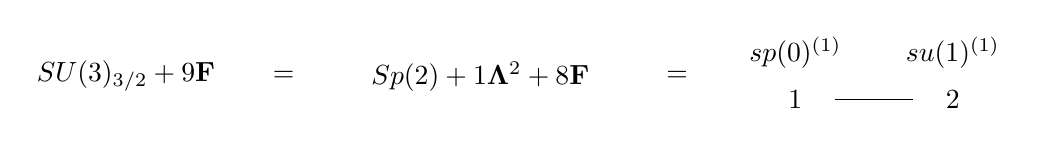
\begin{tikzpicture}
\draw (0, 0) node {$ SU(3)_{3/2} + 9\mathbf{F} $}
(2, 0) node {$ = $}
(4.5, 0) node {$ Sp(2) + 1\mathbf{\Lambda}^2 + 8\mathbf{F} $}
(7, 0) node {$ = $}
(8.5, 0.3) node {$ \mathfrak{sp}(0)^{(1)} $}
(8.5, -0.3) node {$ 1 $}
(10.5, 0.3) node {$ \mathfrak{su}(1)^{(1)} $}
(10.5, -0.3) node {$ 2 $}
(9, -0.3) -- (10, -0.3)
;
\end{tikzpicture}
\end{align}
The geometric construction for this theory is given by
\begin{align}
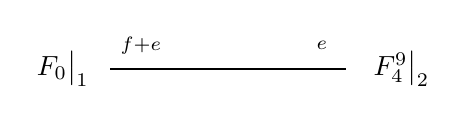
\begin{tikzpicture}
\draw[thick](-3,0)--(0,0);	
\node at(-3.6,0) {$\mathbb{F}_{0}{}\big|_1$};
\node at(-2.6,0.3) {${}_{f+e}$};
\node at(0.7,0) {$\mathbb{F}_{4}^{9}{}\big|_2$};
\node at(-0.3,0.3) {${}_{e}$};
\end{tikzpicture}
\end{align}

The validity of the blowup equations for the 6d rank-2 E-string was checked in \cite{Gu:2019pqj}. Here, we will solve the blowup equations from the perspective of two dual 5d gauge theories. First, the full effective prepotential of the $ SU(3) $ theory on the Coulomb branch where $\phi_2\ge \phi_1>0$ is
\begin{align}
\mathcal{E} & = \frac{1}{\epsilon_1 \epsilon_2} \qty(\mathcal{F} - \frac{\epsilon_1^2 + \epsilon_2^2}{48} \qty(4\phi_1 - 14\phi_2 ) + \epsilon_+^2 (\phi_1 + \phi_2) ) \,, \nonumber \\
6\mathcal{F}
&= 8\phi_1^3 - 3\phi_1^2 \phi_2 - 3\phi_1 \phi_2^2 + 8\phi_2^2 + \frac{9}{2} \phi_1 \phi_2 (\phi_1 - \phi_2) + 6m_0 (\phi_1^2 - \phi_1 \phi_2 + \phi_2^2) \nonumber \\
& \quad - \frac{1}{2} \sum_{i=1}^9 \qty((\phi_2 - m_i)^3 + (\phi_2 - \phi_1 + m_i)^3 + (\phi_1 + m_i)^3) \, ,
\end{align}
where $ m_0 $ is the $SU(3)$ gauge coupling and $ m_{i=1, \cdots, 9} $ are mass parameters of the fundamental hypermultiplets. A set of consistent magnetic fluxes
\begin{align}
n_i \in \mathbb{Z} \, , \quad
B_{m_0} = -3/4 \, , \quad
B_{m_i} = 1/2 \quad (1 \leq i \leq 9) \, .
\end{align}
provides a solvable unity blowup equation. By solving the blowup equation, we obtain the BPS spectrum given in Table~\ref{table:SU3_3/2_9F}.

\begin{table}
	\centering
	\begin{tabular}{|c|C{25ex}||c|C{25ex}|} \hline
		$ \mathbf{d} $ & $ \oplus N_{j_l, j_r}^{\mathbf{d}} (j_l, j_r) $ & $ \mathbf{d} $ & $ \oplus N_{j_l, j_r}^{\mathbf{d}} (j_l, j_r) $ \\ \hline
		$ (1, -1, 0) $ & $ (0, 0) $ & $ (1, -1, 1) $ & $ (0, 1) $ \\ \hline
		$ (1, -1, 2) $ & $ (0, 2) $ & $ (1, -\frac{2}{3}, \frac{2}{3}) $ & $ 9(0, \frac{1}{2}) $ \\ \hline
		$ (1, -\frac{2}{3}, \frac{5}{3}) $ & $ 9(0, \frac{3}{2}) $ & $ (1, -\frac{1}{3}, \frac{1}{3}) $ & $ 36(0, 0) $ \\ \hline
		$ (1, -\frac{1}{3}, \frac{4}{3}) $ & $ 36(0, 1) $ & $ (1, 0, 1) $ & $ (0,0) \oplus 84(0,\frac{1}{2}) \oplus (0,1) $ \\ \hline
		$ (1, 0, 2) $ & $ (0,1) \oplus 84(0,\frac{3}{2}) \oplus (0,2) $ & $ (1, \frac{1}{3}, \frac{2}{3}) $ & $ 126(0,0) \oplus 9(0,\frac{1}{2}) $ \\ \hline
		$ (1, \frac{1}{3}, \frac{5}{3}) $ & $ 9(0,\frac{1}{2}) \oplus 126(0,1) \oplus 9(0,\frac{3}{2}) $ & $ (1, \frac{2}{3}, \frac{1}{3}) $ & $ 45(0,0) $ \\ \hline
		$ (1, \frac{2}{3}, \frac{4}{3}) $ & $ 36(0,0) \oplus 126(0,\frac{1}{2}) \oplus 36(0,1) $ & $ (1, 1, 0) $ & $ (0,0) \oplus (0,\frac{1}{2}) $ \\ \hline
		$ (1, 1, 1) $ & $ 85(0,0) \oplus 85(0,\frac{1}{2})\oplus (0,1) $ & $ (1, 1, 2) $ & $ (0,0) \oplus 84(0,\frac{1}{2}) \oplus 85(0,1) \oplus 84(0,\frac{3}{2}) \oplus (0,2) $ \\ \hline
		$ (2, -1, 1) $ & $ 84(0, 1) $ & $ (2, -\frac{2}{3}, \frac{2}{3}) $ & $ 126(0, \frac{1}{2}) $ \\ \hline
		$ (2, -\frac{1}{3}, \frac{1}{3}) $ & $ 126(0, 0) $ & $ (2, 0, 1) $ & $ 85(0, 0) \oplus 1219(0, \frac{1}{2}) \oplus 85(0, 1) \oplus 84(\frac{1}{2}, 1) $ \\ \hline
		$ (2, \frac{1}{3}, \frac{2}{3}) $ & $ 801(0, 0) \oplus 135(0, \frac{1}{2}) \oplus 36(\frac{1}{2}, \frac{1}{2}) $ & $ (2, \frac{2}{3}, \frac{1}{3}) $ & $ \! 162(0, 0) \oplus 9(0, \frac{1}{2}) \oplus 9(\frac{1}{2}, 0) \! $ \\ \hline
		$ (2, 1, 0) $ & $ (0, 0) \oplus (0, 1) \oplus (\frac{1}{2}, \frac{1}{2}) $ & $ (2, 1, 1) $ & $ 1465(0, 0) \oplus 1387(0, \frac{1}{2}) \oplus 168(0, 1) \oplus (0, 2) \oplus 84(\frac{1}{2}, 0) \oplus 83(\frac{1}{2}, \frac{1}{2}) \oplus 84(\frac{1}{2}, 1) \oplus (\frac{1}{2}, \frac{3}{2}) \oplus (1, 1) $ \\ \hline
	\end{tabular}
	\caption{BPS spectrum of the $ SU(3)_{3/2} + 9\mathbf{F} $ theory for $ d_1 = 1 $, $ d_2 \leq 1 $, $ d_3 \leq 2 $ and $ d_1 = 2 $, $ d_2, d_3 \leq 1 $. All flavor mass parameters $ m_{i=1, \cdots, 9} $ are turned off and $ \mathbf{d} = (d_1, d_2, d_3) $ labels the BPS states with charge $ d_1 m_0 + d_2 \alpha_1 + d_3 \alpha_2 $ for the simple roots $ \alpha_1 $ and $ \alpha_2 $ of $ \mathfrak{su}(3) $ algebra.} \label{table:SU3_3/2_9F}
\end{table}

On the other hand, in the $ Sp(2) $ theory, the full effective prepotential in the same chamber is
\begin{align}
\mathcal{E}& = \frac{1}{\epsilon_1 \epsilon_2} \qty(\mathcal{F} - \frac{\epsilon_1^2 + \epsilon_2^2}{48} \qty(4\phi_1 - 14\phi_2) +  \epsilon_+^2 (\phi_1 + \phi_2) ) \,,  \\
6\mathcal{F}
&= 8\phi_1^3 + 12\phi_1^2 \phi_2 - 18\phi_1 \phi_2^2 + 8\phi_2^3 + m_0 (2\phi_1^2 - 2\phi_1 \phi_2 + \phi_2^2)  \nonumber \\
& \quad - \frac{1}{2} \sum_{i=1}^8 \qty((\phi_1 + m_i)^3 + (-\phi_1 + \phi_2 + m_i)^3 + (-\phi_1 + \phi_2 - m_i)^3 + (\phi_1 - m_i)^3) \nonumber \\
& \quad - \frac{1}{2} \Big((\phi_2 + m_9)^3 + (2\phi_1 - \phi_2 + m_9)^3 + (-2\phi_1 + \phi_2 + m_9)^3 + (\phi_2 - m_9)^3\Big) \nonumber \, ,
\end{align}
where $ m_0 $ is the $Sp(2)$ gauge coupling, $ m_{i=1, \cdots, 8} $ are mass parameters of the $Sp(2)$ fundamentals and $ m_9 $ denotes the mass parameter of the antisymmetric hyper.

The K\"ahler parameters in the $Sp(2)$ theory are mapped to those in the $ SU(3) $ theory as
\begin{align}
\phi_1^{Sp} &= \phi_1^{SU} + \frac{1}{2} m_0^{SU} + \frac{1}{4} \sum_{j=1}^8 m_j^{SU} - \frac{1}{4} m_9^{SU} , \
\phi_2^{Sp} = \phi_2^{SU} + m_0^{SU} + \frac{1}{2} \sum_{j=1}^8 m_j^{SU} - \frac{1}{2} m_9^{SU}\ , \nonumber \\
m_0^{Sp} &= \frac{3}{2} m_0^{SU} + \frac{1}{4} \sum_{i=1}^9 m_i^{SU} , \ 
m_i^{Sp} = \frac{1}{2} m_0^{SU} - m_i^{SU} + \frac{1}{4} \sum_{j=1}^8 m_j^{SU} - \frac{1}{4} m_9^{SU} \ (1 \leq i \leq 7)\ ,  \nonumber \\
m_8^{Sp} &= -\frac{1}{2} m_0^{SU} + m_8^{SU} - \frac{1}{4} \sum_{j=1}^8 m_j^{SU} + \frac{1}{4} m_9^{SU} , \ \
m_9^{Sp} = m_0^{SU} + \frac{1}{2} \sum_{j=1}^9 m^{SU}_j \, .
\end{align}

In the $Sp(2)$ frame, we find a set of consistent magnetic fluxes
\begin{align}
n_i \in \mathbb{Z} \, , \quad
B_{m_0} = 0 \, , \quad
B_{m_i} = 1/2 \quad  (1 \leq i \leq 9) \, .
\end{align}
This leads to a solvable unity blowup equation. We have checked that the solution to the blowup equation agrees with the BPS spectrum of the dual $SU(3)$ gauge theory given in Table~\ref{table:SU3_3/2_9F}.

The instanton partition function of the $ Sp(2) + 1\mathbf{\Lambda}^2 + 8\mathbf{F} $ theory can also be calculated using the ADHM construction introduced in \cite{Aharony:1997pm, Kim:2012gu, Hwang:2014uwa}. We checked that our result from the blowup formula is in perfect agreement with the ADHM result in the K\"ahler parameter expansion.


\subsubsection{\texorpdfstring{$SU(3)_0+10\mathbf{F}$, $Sp(2)+10\mathbf{F}$}{SU(3)0 + 10F}}

The 5d $ SU(3)_0 + 10\mathbf{F} $ theory and the $ Sp(2) + 10\mathbf{F} $ theory are two dual 5d descriptions for the KK theory arising from the circle compactification of the 6d $ Sp(1) $ gauge theory with 10 fundamental hypermultiplets,
\begin{align}
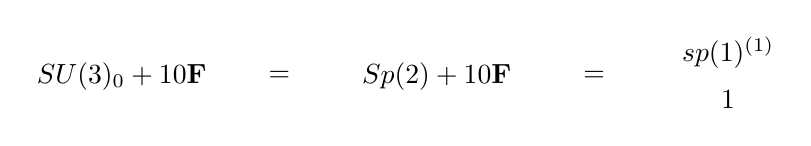
\begin{tikzpicture}
\draw (0, 0) node {$ SU(3)_{0} + 10\mathbf{F} $}
(2, 0) node {$ = $}
(4, 0) node {$ Sp(2) + 10\mathbf{F} $}
(6, 0) node {$ = $}
(7.7, 0.3) node {$ \mathfrak{sp}(1)^{(1)} $}
(7.7, -0.3) node {$ 1 $}
;
\end{tikzpicture}
\end{align}
This theory is geometrically engineered by gluing $ \mathbb{F}_6^{10} $ and $ \mathbb{F}_0 $ \cite{Jefferson:2018irk}.
\begin{align}
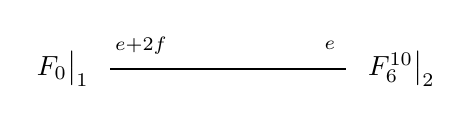
\begin{tikzpicture}
\draw[thick](-3,0)--(0,0);	
\node at(-3.6,0) {$\mathbb{F}_{0}{}\big|_1$};
\node at(-2.6,0.3) {${}_{e+2f}$};
\node at(0.7,0) {$\mathbb{F}_{6}^{10}{}\big|_2$};
\node at(-0.2,0.3) {${}_{e}$};
\end{tikzpicture}
\end{align}
The blowup equation for this theory from the 6d gauge theory perspective was checked to be satisfied by substituting the known one-string elliptic genus into the blowup equation  in \cite{Gu:2020fem}.

We will now compute the BPS spectrum of this theory using the blowup equations in the 5d gauge theory descriptions. First, the full prepotential of the $SU(3)$ gauge theory on the chamber $\phi_2\ge \phi_1>0$ is
\begin{align}
\mathcal{E} &= \frac{1}{\epsilon_1 \epsilon_2} \qty(\mathcal{F} - \frac{\epsilon_1^2 + \epsilon_2^2}{48} \qty(4\phi_1 - 16\phi_2 ) + \epsilon_+^2 (\phi_1 + \phi_2) ) \,, \nonumber \\
6\mathcal{F}
&= 8\phi_1^3 - 3\phi_1^2 \phi_2 - 3\phi_1 \phi_2^2 + 8\phi_2^2 + 6m_0 (\phi_1^2 - \phi_1 \phi_2 + \phi_2^2) \nonumber \\
& \quad - \frac{1}{2} \sum_{i=1}^{10} \qty((\phi_2 - m_i)^3 + (\phi_2 - \phi_1 + m_i)^3 + (\phi_1 + m_i)^3) \, .
\end{align}
We find a set of consistent magnetic fluxes
\begin{align}
n_i \in \mathbb{Z} \, , \ \
B_{m_0} = 0 \, , \ \
B_{m_i} = 1/2 \ \ (1 \leq i \leq 5) \, , \ \ 
B_{m_i} = -1/2 \ \ (6 \leq i \leq 10) \ ,
\end{align}
which provides a solvable unity blowup equation.

In the $ Sp(2) $ gauge theory, on the other hand, the full effective prepotential on the same chamber takes the form of
\begin{align}
\mathcal{E}
&= \frac{1}{\epsilon_1 \epsilon_2} \qty(\mathcal{F} - \frac{\epsilon_1^2 + \epsilon_2^2}{48} (4\phi_1 - 16\phi_2) + \epsilon_+^2 (\phi_1 + \phi_2)) \,, \nonumber \\
6\mathcal{F}
&= 8\phi_1^3 + 12\phi_1^2 \phi_2 - 18\phi_1 \phi_2^2 + 8\phi_2^3 + m_0(2\phi_1^2 - 2\phi_1 \phi_2 + \phi_2^2)  \nonumber\\
& \quad - \frac{1}{2}\sum_{i=1}^{10} \qty((\phi_1 \pm m_i)^3 + (-\phi_1 + \phi_2 \pm m_i)^3 )\,,  
\end{align}
where $ m_0 $ is the $ Sp(2) $ gauge coupling and $ m_{i=1, \cdots, 10} $ are mass parameters of the fundamental hypers. 
One possible choice of consistent magnetic fluxes in the $Sp(2)$ theory is
\begin{align}
n_i \in \mathbb{Z} \, , \quad
B_{m_0} = 0 \, , \quad
B_{m_i} = 1/2 \quad (1 \leq i \leq 10) \ .
\end{align}
The K\"ahler parameters in two 5d theories are mapped to each other by the relations \cite{Hayashi:2016abm}
\begin{align}
\phi_1^{Sp} &= \phi_1^{SU} + \frac{1}{2}m_0^{SU} + \frac{1}{4}\sum_{i=1}^{10} m_i^{SU} \,, \ \
\phi_2^{Sp} = \phi_2^{SU} + m_0^{SU} + \frac{1}{2}\sum_{i=1}^{10} m_i^{SU} \,, \ \ m_0^{Sp} = m_0^{SU} \,, \nonumber \\
m_i^{Sp} &= \frac{1}{2} m_0^{SU} - m_j^{SU} + \frac{1}{4}\sum_{j=1}^{10} m_j^{SU} \quad (1 \leq i \leq 9) \,, \ \
m_{10}^{Sp} = -\frac{1}{2} m_0^{SU} - \frac{1}{4}\sum_{j=1}^{9} m_j^{SU} + \frac{3}{4} m_{10}^{SU} .
\end{align} 

We list in Table~\ref{table:sp2_10F} some leading BPS states computed by solving the blowup equation in the $ Sp(2) + 10\mathbf{F} $ theory.
We checked that this solution agrees with the result from the  $ SU(3)_0 + 10\mathbf{F} $ description and also agree with the ADHM result for the $ Sp(2) + 10\mathbf{F} $ theory computed in \cite{Yun:2016yzw} as well as topological vertex \cite{Hayashi:2016abm} in series expansion of K\"ahler parameters.
\begin{table}
	\centering
	\begin{tabular}{|c|C{25ex}||c|C{25ex}|} \hline
		$ \mathbf{d} $ & $ \oplus N_{j_l, j_r}^{\mathbf{d}} (j_l, j_r) $ & $ \mathbf{d} $ & $ \oplus N_{j_l, j_r}^{\mathbf{d}} (j_l, j_r) $ \\ \hline
		$ (1, 1, 1) $ & $ 512(0, 0) $ & $ (1, 1, \frac{3}{2}) $ & $ 512(0, \frac{1}{2}) $ \\ \hline
		$ (1, 1, 2) $ & $ 512(0, 1) $ & $ (1, 2, \frac{3}{2}) $ & $ 512(0, \frac{1}{2}) $ \\ \hline
		$ (1, 2, 2) $ & $ 512(0, 0) \oplus 512(0, 1) $ & $ (2, 0, -1) $ & $ (0, \frac{1}{2}) $ \\ \hline
		$ (2, 0, -\frac{1}{2}) $ & $ 20(0, 0) $ & $ (2, 0, \frac{1}{2}) $ & $ 20(0, 0) $ \\ \hline
		$ (2, 0, 1) $ & $ (0, \frac{1}{2}) $ & $ (2, 1, -1) $ & $ (0, \frac{3}{2}) $ \\ \hline
		$ (2, 1, -\frac{1}{2}) $ & $ 20(0, 1) $ & $ (2, 1, 0) $ & $ 192(0, \frac{1}{2}) \oplus (0, \frac{3}{2}) \oplus (\frac{1}{2}, 0) \oplus (\frac{1}{2}, 1) $ \\ \hline
		$ (2, 1, \frac{1}{2}) $ & $ 1180(0, 0) \oplus 20(0, 1) \oplus 20(\frac{1}{2}, \frac{1}{2}) $ & $ (2, 1, 1) $ & $ 192(0, \frac{1}{2}) \oplus (0, \frac{3}{2}) \oplus (\frac{1}{2}, 0) \oplus (\frac{1}{2}, 1) $ \\ \hline
		$ (2, 2, -1) $ & $ (0, \frac{5}{2}) $ & $ (2, 2, -\frac{1}{2}) $ & $ 20(0, 2) $ \\ \hline
		$ (2, 2, 0) $ & $ (0, \frac{1}{2}) \oplus 192(0, \frac{3}{2}) \oplus (0, \frac{5}{2}) \oplus (\frac{1}{2}, 1) \oplus (\frac{1}{2}, 2) $ & $ (2, 1, \frac{1}{2}) $ & $ 20(0, 0) \oplus 1180(0, 1) \oplus 20(0, 2) \oplus 20(\frac{1}{2}, \frac{1}{2}) \oplus 20(\frac{1}{2}, \frac{3}{2}) $ \\ \hline
		$ (2, 2, 1) $ & \multicolumn{3}{C{65ex}|}{$ 5230(0, \frac{1}{2}) \oplus 192(0, \frac{3}{2}) \oplus (0, \frac{5}{2}) \oplus 192(\frac{1}{2}, 0) \oplus 193(\frac{1}{2}, 1) \oplus (\frac{1}{2}, 2) \oplus (1, \frac{1}{2}) \oplus (1, \frac{3}{2}) $} \\ \hline
	\end{tabular}
	\caption{BPS spectrum of the $ Sp(2) + 10\mathbf{F} $ theory for $ d_1 = 1 $, $ d_2, d_3 \leq 2 $ and $ d_1 = 2 $, $ d_2 \leq 2 $, $ d_3 \leq 1 $. Here, $ \mathbf{d} = (d_1, d_2, d_3) $ labels BPS states with charge $ d_1 m_0 + d_2 \alpha_1 + d_3 \alpha_2 $, where $ \alpha_1 = 2\phi_1 - \phi_2 $, $ \alpha_2 = -2\phi_1 + 2\phi_2 $ are the simple roots of $ \mathfrak{sp}(2) $ algebra, and 10 flavor charges are blindly summed over.} \label{table:sp2_10F}
\end{table}


\subsubsection{\texorpdfstring{$SU(2)\times SU(2)+2\,\mathbf{bi\text{-}F}$}{SU(2)*SU(2) + 2bifund}}

We will now give an example for 5d quiver gauge theories. The 5d theory with $SU(2)\times SU(2)$ gauge group and 2 bi-fundamental hypermultiplets ($\mathbf{bi\text{-}F}$) is the KK theory obtained from a circle compactification of the 6d $SU(2)$ gauge theory with 4 fundamental hypermultiplets.

The full effective prepotential of the $ SU(2) \times SU(2) $ gauge theory on the Coulomb branch where $\phi_2\ge\phi_1>0$ is given by
\begin{align}
\mathcal{E}
&= \frac{1}{\epsilon_1 \epsilon_2} \qty(\mathcal{F} - \frac{\epsilon_1^2 + \epsilon_2^2}{12} \qty(\phi_1 - \phi_2) + \epsilon_+^2 (\phi_1 + \phi_2) ) \,,  \\
6\mathcal{F}
&= 8\phi_1^3 + 8\phi_2^3 + 6m_1 \phi_1^2 + 6m_2 \phi_2^2 - \frac{1}{2}\sum_{i=3}^4\Big((\phi_1 + \phi_2 \pm m_i)^3 + (-\phi_1 + \phi_2 \pm m_i)^3 \Big) \ , \nonumber
\end{align}
where $ m_1 $ and $ m_2 $ are the gauge couplings for two $ SU(2) $ gauge groups respectively, while $ m_3$ and $m_4 $ are the mass parameters of two bi-fundamentals. 

A unity blowup equation can be formulated with a set of the consistent magnetic fluxes given by
\begin{align}
n_i \in \mathbb{Z} \ , \quad
B_{m_1} = 0 \ , \quad
B_{m_2} = 0 \ , \quad
B_{m_{3,4}} = 1/2 \ .
\end{align}
The solution to the blowup equation is given in Table~\ref{table:SU2_bifund}. We also computed the partition function of this theory using the ADHM method and confirmed that the result agrees with the BPS spectrum in Table~\ref{table:SU2_bifund}. 

\begin{table}
	\centering
	\begin{tabular}{|c|C{21ex}||c|C{21ex}|} \hline
		$ \mathbf{d} $ & $ \oplus N_{j_l, j_r}^{\mathbf{d}} (j_l, j_r) $ & $ \mathbf{d} $ & $ \oplus N_{j_l, j_r}^{\mathbf{d}} (j_l, j_r) $ \\ \hline
		$ (1, 0, 1, -1, -1) $ & $ 2(0, 0) $ & $ (1, 0, 1, 1, -1) $ & $ 2(0, 0) $ \\ \hline
		$ (1, 0, 2, -2, 0) $ & $ (0, \frac{1}{2}) $ & $ (1, 0, 2, 0, -2) $ & $ (0, \frac{1}{2}) $ \\ \hline
		$ (1, 0, 2, 0, 0) $ & $ 4(0, \frac{1}{2}) $ & $ (1, 0, 2, 2, 0) $ & $ (0, \frac{1}{2}) $ \\ \hline
		$ (1, 1, -1, 1, -1) $ & $ 2(0, 0) $ & $ (1, 1, 0, 2, -2) $ & $ 4(0, \frac{1}{2}) $ \\ \hline
		$ (1, 1, 0, 2, 0) $ & $ 10(0, \frac{1}{2}) \oplus (0, \frac{3}{2}) \oplus (\frac{1}{2}, 0) \oplus (\frac{1}{2}, 1) $ & $ (1, 1, 1, -1, -1) $ & $ 2(0, 0) $ \\ \hline
		$ (1, 1, 1, 1, -3) $ & $ 2(0, 0) $ & $ (1, 1, 1, 1, -1) $ & $ 14(0, 0) \oplus 4(0, 1) \oplus 2(\frac{1}{2}, \frac{1}{2}) $ \\ \hline
		$ (1, 1, 2, 0, -2) $ & $ 4(0, \frac{1}{2}) $ & $ (1, 1, 2, 0, 0) $ & $ 10(0, \frac{1}{2}) \oplus (0, \frac{3}{2}) \oplus (\frac{1}{2}, 0) \oplus (\frac{1}{2}, 1) $ \\ \hline
		$ (1, 1, 2, 2, -2) $ & $ 10(0, \frac{1}{2}) \oplus 5(0, \frac{3}{2}) \oplus (\frac{1}{2}, 0) \oplus (\frac{1}{2}, 1) $ & $ (1, 1, 2, 2, 0) $ & $ 25(0, \frac{1}{2}) \oplus 14(0, \frac{3}{2}) \oplus (0, \frac{5}{2}) \oplus 4(\frac{1}{2}, 0) \oplus 5(\frac{1}{2}, 1) \oplus (\frac{1}{2}, 2) $ \\ \hline
	\end{tabular}
	\caption{BPS spectrum of the $ SU(2) \times SU(2) $ theory with $ 2 $ bifundamentals. Here, $ \mathbf{d}=(d_1, d_2, d_3, d_4, d_5) $ labels the BPS states with charge $ d_1 m_1 + d_2 m_2 + d_3 \phi_1 + d_4 \phi_2 + d_5 m_i $ where $d_5$ counts collective degrees of two bi-fundamental matters with masses $m_{i=3,4}$. There is a symmetry exchanging $ (d_1, d_2, d_3, d_4, d_5) \leftrightarrow (d_2, d_1, d_4, d_3, d_5) $ and $ d_5 \leftrightarrow -d_5 $, so we list BPS states up to $ (d_3, d_4) \leq (2, 2) $ and $ d_5 \leq 0 $ for $ (1, 0) $ and $ (1, 1) $ instantons.} \label{table:SU2_bifund}
\end{table}


\subsubsection{\texorpdfstring{$ SU(3)_0 + 1\mathbf{Adj} $}{SU(3)0 + 1Adj}}

The 5d $ SU(3)_0 $ gauge theory with one adjoint hypermultiplet is equivalent to a circle reduction of the 6d $ \mathcal{N}=(2, 0) $ $ A_2$ theory \cite{Bhardwaj:2019fzv},
\begin{align}
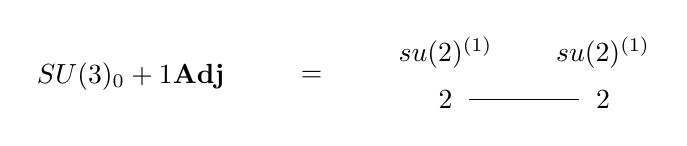
\begin{tikzpicture}
\draw (0, 0) node {$ SU(3)_0 + 1\mathbf{Adj} $}
(2.3, 0) node {$ = $}
(4, 0.3) node {$ \mathfrak{su}(2)^{(1)} $}
(4, -0.3) node {$ 2 $}
(6, 0.3) node {$ \mathfrak{su}(2)^{(1)} $}
(6, -0.3) node {$ 2 $}
(4.3, -0.3) -- (5.7, -0.3);
\end{tikzpicture}
\end{align}
The cubic prepotential of this theory on the chamber where $2\phi_2>\phi_1 > \frac{1}{2}\phi_2$ is
\begin{align}
6\mathcal{F}
&= 8\phi_1^3 - 3\phi_1^2 \phi_2 - 3\phi_1 \phi_2^2 + 8\phi_2^3 + 6m_0 (\phi_1^2 - \phi_1 \phi_2 + \phi_2^2) \nonumber \\
& \quad - \frac{1}{2}\Big((\phi_1 + \phi_2 \pm m_1)^3 + (-\phi_1 + 2\phi_2 \pm m_1)^3 + (2\phi_1 - \phi_2 \pm m_1)^3 \Big),
\end{align}
where $ m_0 $ is the gauge coupling and $ m_1 $ is the mass parameter of the adjoint matter. The effective prepotential is
\begin{align}
\mathcal{E}
= \frac{1}{\epsilon_1 \epsilon_2} \qty(\mathcal{F} + \epsilon_+^2 (\phi_1 + \phi_2)) \ .
\end{align}

We find that a set of consistent magnetic fluxes
\begin{align}
n_i \in \mathbb{Z} \ , \quad
B_{m_0} = 0 \ , \quad
B_{m_1} = 1/2 \ 
\end{align}
gives rise to a solvable unity blowup equation.
The BPS spectrum obtained by solving the blowup equation is listed in Table~\ref{table:su3_adj}. We also computed the instanton partition function for $ SU(3)_0 + 1\mathbf{Adj}$ independently using the ADHM construction and confirmed that our result agrees with the result from the ADHM method.

\begin{table}
	\centering
	\begin{tabular}{|c|C{25ex}||c|C{25ex}|} \hline
		$ \mathbf{d} $ & $ \oplus N_{j_l, j_r}^{\mathbf{d}} (j_l, j_r) $ & $ \mathbf{d} $ & $ \oplus N_{j_l, j_r}^{\mathbf{d}} (j_l, j_r) $ \\ \hline
		$ (1, 0, 1, -2) $ & $ (0, \frac{1}{2}) $ & $ (1, 0, 1, -1) $ & $ (0, 0) \oplus (0, 1) \oplus (\frac{1}{2}, \frac{1}{2}) $ \\ \hline
		$ (1, 0, 1, 0) $ & $ 2(0, \frac{1}{2}) \oplus (\frac{1}{2}, 0) \oplus (\frac{1}{2}, 1) $ & $ (1, 0, 2, -2) $ & $ (0, \frac{3}{2}) $ \\ \hline
		$ (1, 0, 2, -1) $ & $ (0, 1) \oplus (0, 2) \oplus (\frac{1}{2}, \frac{3}{2}) $ & $ (1, 0, 2, 0) $ & $ 2(0, \frac{3}{2}) \oplus (\frac{1}{2}, 1) \oplus (\frac{1}{2}, 2) $ \\ \hline
		$ (1, 1, 1, -3) $ & $ (0, 0) $ & $ (1, 1, 1, -2) $ & $ 3(0, \frac{1}{2}) \oplus (\frac{1}{2}, 0) $ \\ \hline
		$ (1, 1, 1, -1) $ & $ 5(0, 0) \oplus 2(0, 1) \oplus 3(\frac{1}{2}, \frac{1}{2}) $ & $ (1, 1, 1, 0) $ & $ 6(0, \frac{1}{2}) \oplus 4(\frac{1}{2}, 0) \oplus 2(\frac{1}{2}, 1) $ \\ \hline
		$ (1, 1, 2, -3) $ & $ (0, 1) $ & $ (1, 1, 2, -2) $ & $ 2(0, \frac{1}{2}) \oplus 2(0, \frac{3}{2}) \oplus (\frac{1}{2}, 1) $ \\ \hline
		$ (1, 1, 2, -1) $ & $ (0,0) \oplus 5(0,1) \oplus (0,2) \oplus 2(\frac{1}{2},\frac{1}{2}) \oplus 2(\frac{1}{2},\frac{3}{2}) $ & $ (1, 1, 2, 0) $ & $ 4(0,\frac{1}{2}) \oplus 4(0,\frac{3}{2}) \oplus (\frac{1}{2},0) \oplus 4(\frac{1}{2},1) \oplus (\frac{1}{2},2) $ \\ \hline
		$ (1, 2, 2, -3) $ & $ (0, 0) \oplus (0, 1) $ & $ (1, 2, 2, -2) $ & $ 4(0,\frac{1}{2}) \oplus 3(0,\frac{3}{2}) \oplus (\frac{1}{2},0) \oplus (\frac{1}{2},1) $ \\ \hline
		$ (1, 2, 2, -1) $ & $ 5(0,0) \oplus 7(0,1) \oplus 2(0,2) \oplus 4(\frac{1}{2},\frac{1}{2}) \oplus 3(\frac{1}{2},\frac{3}{2}) $ & $ (1, 2, 2, 0) $ & $ 8(0,\frac{1}{2}) \oplus 6(0,\frac{3}{2}) \oplus 4(\frac{1}{2},0) \oplus 6(\frac{1}{2},1) \oplus 2(\frac{1}{2},2) $ \\ \hline
		$ (2, 0, 1, -3) $ & $ (0, 0) $ & $ (2, 0, 1, -2) $ & $ 2(0, \frac{1}{2}) \oplus (\frac{1}{2}, 0) \oplus (\frac{1}{2}, 1) $ \\ \hline
		$ (2, 0, 1, -1) $ & $ 4(0, 0) \oplus 2(0, 1) \oplus 3(\frac{1}{2}, \frac{1}{2}) \oplus (\frac{1}{2}, \frac{3}{2}) \oplus (1, 1) $ & $ (2, 0, 1, 0) $ & $ 5(0,\frac{1}{2}) \oplus (0,\frac{3}{2}) \oplus 3(\frac{1}{2},0) \oplus 3(\frac{1}{2},1) \oplus (1,\frac{1}{2}) \oplus (1,\frac{3}{2}) $ \\ \hline
		$ (2, 1, 1, -3) $ & $ 5(0,0) \oplus 2(0,1) \oplus 3(\frac{1}{2},\frac{1}{2}) $ & $ (2, 1, 1, -2) $ & $ 14(0,\frac{1}{2}) \oplus (0,\frac{3}{2}) \oplus 9(\frac{1}{2},0) \oplus 7(\frac{1}{2},1) \oplus 2(1,\frac{1}{2}) $ \\ \hline
		$ (2, 1, 1, -1) $ & $ 22(0,0) \oplus 14(0,1) \oplus 22(\frac{1}{2},\frac{1}{2}) \oplus 4(\frac{1}{2},\frac{3}{2}) \oplus 4(1,0) \oplus 5(1,1) $ & $ (2, 1, 1, 0) $ & $ 31(0,\frac{1}{2}) \oplus 5(0,\frac{3}{2}) \oplus 21(\frac{1}{2},0) \oplus 17(\frac{1}{2},1) \oplus 9(1,\frac{1}{2}) \oplus 3(1,\frac{3}{2}) $ \\ \hline
	\end{tabular}
	\caption{BPS spectrum of $ SU(3)_0 + 1\mathbf{Adj} $ theory for $ d_1 = 1 $, $ d_2, d_3 \leq 2 $ and $ d_1 = 2 $, $ d_2, d_3 \leq 1 $. Here $ \mathbf{d} = (d_1, d_2, d_3, d_4) $ labels the BPS states with charge $ d_1 m_0 + d_2 \alpha_1 + d_3 \alpha_2 + d_4 m_1 $, where $ \alpha_1 $ and $ \alpha_2 $ are simple roots of $ \mathfrak{su}(3) $ algebra. The states related by the symmetries $ d_2 \leftrightarrow d_3 $ and $ d_4 \leftrightarrow -d_4 $ are omitted.} \label{table:su3_adj}
\end{table}


\subsubsection{\texorpdfstring{$Sp(2)_0+1\mathbf{Adj}$}{Sp(2)0 + 1Adj}}

There are two $Sp(2)_\theta$ gauge theories with an adjoint hypermultiplet in 5d distinguished by two distinct theta angles $\theta=0$ or $\theta=\pi$. In this subsection, we discuss the case with $\theta= 0$.

The 5d $ Sp(2)_0 + 1\mathbf{Adj} $ theory is the KK-theory obtained by the $ \mathbb{Z}_2 $ twisted compactification of the 6d $ \mathcal{N} = (2, 0) $ $A_3$ theory \cite{Tachikawa:2011ch},
\begin{align}
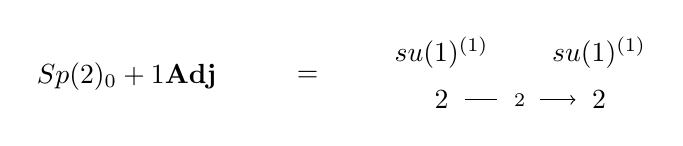
\begin{tikzpicture}
\draw (0, 0) node {$ Sp(2)_0 + 1\mathbf{Adj} $}
(2.3, 0) node {$ = $}
(4, 0.3) node {$ \mathfrak{su}(1)^{(1)} $}
(4, -0.3) node {$ 2 $}
(6, 0.3) node {$ \mathfrak{su}(1)^{(1)} $}
(6, -0.3) node {$ 2 $}
(4.3, -0.3) -- (4.7, -0.3)
(5, -0.3) node {$ _2 $}
;
\draw [->] (5.25, -0.3) -- (5.7, -0.3);
\end{tikzpicture}
\end{align}
This is a non-geometric theory. This theory on the other hand has a 5-brane web realization with an $O7^+$ plane (or frozen singularity) which will be discussed in Appendix~\ref{sec:appendix2}. 

The BPS spectrum of this theory can be obtained by solving the blowup equation as follows. The full effective prepotential of this theory on the chamber where $2\phi_1>\phi_2>\phi_1>0$ is
\begin{align}\label{eq:Sp2_0_adj_F}
\mathcal{E} & = \frac{1}{\epsilon_1 \epsilon_2} \qty(\mathcal{F} - \frac{\epsilon_1^2 + \epsilon_2^2}{48} \qty(4\phi_1 - 2\phi_2) + \epsilon_+^2 (\phi_1 + \phi_2) ) \,, \nonumber \\
6\mathcal{F}
&= 8\phi_1^3 + 12\phi_1^2 \phi_2 - 18\phi_1 \phi_2^2 + 8\phi_2^3 + m_0 (2\phi_1^2 - 2\phi_1 \phi_2 + \phi_2^2) \\
& \quad -\frac{1}{2} \qty((2\phi_1 \pm m_1)^3 + (\phi_2 \pm m_1)^3 + (-2\phi_1 + 2\phi_2 \pm m_1)^3 + (\pm(2\phi_1 - \phi_2) + m_1)^3), \nonumber
\end{align}
where $ m_0 $ is the gauge coupling and $ m_1 $ is the adjoint mass parameter. One can choose the consistent magnetic fluxes as
\begin{align} \label{eq:Sp2_0_adj_shift}
n_i \in \mathbb{Z} \ , \quad
B_{m_0} = 0 \ , \quad
B_{m_1} = 1/2 \ ,
\end{align}
and formulate a unity blowup equation. The solution to the blowup equation is given in Table~\ref{table:Sp2_0_1Adj}. We checked that this result matches the instanton partition function of the 5d $\mathcal{N}=2$ $Sp(2)_0$ gauge theory computed in \cite{Nekrasov:2004vw,Shadchin:2004yx} using the ADHM construction.
\begin{table}
	\centering
	\begin{tabular}{|c|C{25ex}||c|C{25ex}|} \hline
		$ \mathbf{d} $ & $ \oplus N_{j_l, j_r}^{\mathbf{d}} (j_l, j_r) $ & $ \mathbf{d} $ & $ \oplus N_{j_l, j_r}^{\mathbf{d}} (j_l, j_r) $ \\ \hline
		$ (1, 0, 1, -2) $ & $ (0, \frac{1}{2}) $ & $ (1, 0, 1, -1) $ & $ (0,0) \oplus (0,1) \oplus (\frac{1}{2},\frac{1}{2}) $ \\ \hline
		$ (1, 0, 1, 0) $ & $ 2(0,\frac{1}{2}) \oplus (\frac{1}{2},0) \oplus	(\frac{1}{2},1) $ & $ (1, 0, 2, -2) $ & $ (0, \frac{3}{2}) $ \\ \hline
		$ (1, 0, 2, -1) $ & $ (0,1) \oplus (0,2) \oplus (\frac{1}{2},\frac{3}{2}) $ & $ (1, 0, 2, 0) $ & $ 2(0,\frac{3}{2}) \oplus (\frac{1}{2},1) \oplus (\frac{1}{2},2) $ \\ \hline
		$ (1, 1, 1, -3) $ & $ (0, 0) $ & $ (1, 1, 1, -2) $ & $ 2(0,\frac{1}{2}) \oplus (\frac{1}{2},0) $ \\ \hline
		$ (1, 1, 1, -1) $ & $ 4(0,0) \oplus (0,1) \oplus 2(\frac{1}{2},\frac{1}{2}) $ & $ (1, 1, 1, 0) $ & $ 4(0,\frac{1}{2}) \oplus 3(\frac{1}{2},0) \oplus	(\frac{1}{2},1) $ \\ \hline
		$ (2, 0, 1, -2) $ & $ 2(0,\frac{1}{2}) \oplus (\frac{1}{2},0) \oplus (\frac{1}{2},1) $ & $ (2, 0, 1, -1) $ & $ 4(0,0) \oplus 2(0,1) \oplus 3(\frac{1}{2},\frac{1}{2}) \oplus (\frac{1}{2},\frac{3}{2}) \oplus (1,1) $ \\ \hline
		$ (2, 0, 1, 0) $ & $ 5(0,\frac{1}{2}) \oplus (0,\frac{3}{2}) \oplus	3(\frac{1}{2},0) \oplus 3(\frac{1}{2},1) \oplus	(1,\frac{1}{2}) \oplus (1,\frac{3}{2}) $ & $ (2, 1, 0, -2) $ & $ (0, \frac{1}{2}) $ \\ \hline
		$ (2, 1, 0, -1) $ & $ (0,0) \oplus (0,1) \oplus (\frac{1}{2},\frac{1}{2}) $ & $ (2, 1, 0, 0) $ & $ 2(0,\frac{1}{2}) \oplus (\frac{1}{2},0) \oplus (\frac{1}{2},1) $ \\ \hline
		$ (2, 1, 1, -3) $ & $ 2(0,0) \oplus (\frac{1}{2},\frac{1}{2}) $ & $ (2, 1, 1, -2) $ & $ 6(0,\frac{1}{2}) \oplus 4(\frac{1}{2},0) \oplus	2(\frac{1}{2},1) \oplus (1,\frac{1}{2}) $ \\ \hline
		$ (2, 1, 1, -1) $ & $ 11(0,0) \oplus 5(0,1) \oplus 10(\frac{1}{2},\frac{1}{2}) \oplus (\frac{1}{2},\frac{3}{2}) \oplus 2(1,0) \oplus 2(1,1) $ & $ (2, 1, 1, 0) $ & $ 14(0,\frac{1}{2}) \oplus (0,\frac{3}{2}) \oplus 11(\frac{1}{2},0) \oplus 7(\frac{1}{2},1) \oplus 4(1,\frac{1}{2}) \oplus (1,\frac{3}{2}) $ \\ \hline
	\end{tabular}
	\caption{BPS spectrum of  the $ Sp(2)_{0} + 1\mathbf{Adj} $ theory for $ d_1 = 1, 2 $ and $ d_2 \leq 1 $, $ d_3 \leq 1 $. Here, $ \mathbf{d} = (d_1, d_2, d_3, d_4) $ labels the BPS states with charge $ d_1 m_0 + d_2 \alpha_1 + d_3 \alpha_2 + d_4 m_1 $ where $ \alpha_1 = 2\phi_1 - \phi_2 $, $ \alpha_2 = -2\phi_1 + 2\phi_2 $ are simple roots of $ \mathfrak{sp}(2) $ algebra. The theory has a symmetry exchanging $ d_4 \leftrightarrow -d_4 $ which provides BPS states with flipped charge $d_4\rightarrow -d_4$.} \label{table:Sp2_0_1Adj}
\end{table}


\subsubsection{\texorpdfstring{$SU(3)_{\frac{3}{2}}+1\mathbf{Sym}$, $Sp(2)_\pi+1\mathbf{Adj}$}{SU(3)3/2 + 1Sym}}

The 5d $ Sp(2)_\pi + 1\mathbf{Adj} $ theory is the KK-theory obtained by $ \mathbb{Z}_2 $ twisted compactification of the 6d $ \mathcal{N}=(2, 0) $ $ A_4 $ theory. This theory is also dual to the $ SU(3)_{3/2} + 1\mathbf{Sym} $ theory \cite{Jefferson:2017ahm},
\begin{align}
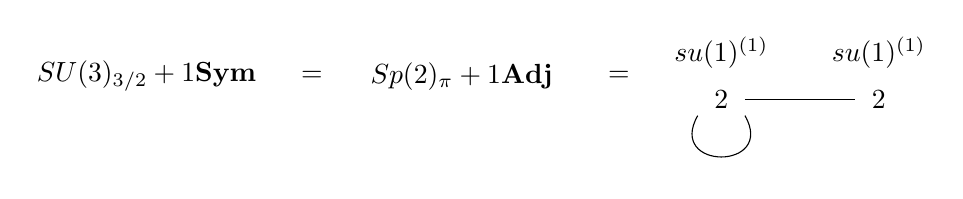
\begin{tikzpicture}
\draw (0, 0) node {$ SU(3)_{3/2} + 1\mathbf{Sym} $}
(2.1, 0) node {$ = $}
(4, 0) node {$ Sp(2)_\pi + 1\mathbf{Adj} $}
(6, 0) node {$ = $}
(7.3, 0.3) node {$ \mathfrak{su}(1)^{(1)} $}
(7.3, -0.3) node {$ 2 $}
(9.3, 0.3) node {$ \mathfrak{su}(1)^{(1)} $}
(9.3, -0.3) node {$ 2 $}
(7.6, -0.3) -- (9.0, -0.3);
\draw (7.0, -0.5) .. controls (6.6, -1.2) and (8.0, -1.2) .. (7.6, -0.5);
\end{tikzpicture}
\end{align}
This theory has no geometric construction, but it can be realized by a 5-brane web with an $O7^+$ plane as discussed in \cite{Hayashi:2018lyv}. See also Appendix~\ref{sec:appendix2} for more details. 

In the $ SU(3) $ description, the effective prepotential on the Coulomb branch where $\phi_2\ge \phi_1>0$ is given by
\begin{align}
\mathcal{E} & = \frac{1}{\epsilon_1 \epsilon_2} \qty(\mathcal{F} - \frac{\epsilon_1^2 + \epsilon_2^2}{48} \qty(4\phi_1 - 2\phi_2) + \epsilon_+^2 (\phi_1 + \phi_2) ) \,, \nonumber \\
6\mathcal{F}
&= 8\phi_1^3 - 3\phi_1^2 \phi_2 - 3\phi_1 \phi_2^2 + 8\phi_2^2 + \frac{9}{2} \phi_1 \phi_2 (\phi_1 - \phi_2) + m_0 (\phi_1^2 - \phi_1 \phi_2 + \phi_2^2) \nonumber \\
& \quad - \frac{1}{2} \big( (2\phi_1 + m_1)^3 + (\phi_2 + m_1)^3 + (-2\phi_1 + 2\phi_2 + m_1)^3 \nonumber \\
& \qquad \qquad + (-\phi_1 + \phi_2 - m_1)^3 + (\phi_1 - m_1)^3 + (2\phi_2 - m_1)^3 \big) \ ,
\end{align}
where $ m_0 $ is the gauge coupling and $ m_1 $ is the mass parameter of the symmetric matter. The following magnetic fluxes give a solvable unity blowup equation for this theory, 
\begin{align}\label{eq:su3_sym_flux}
n_i \in \mathbb{Z} \, , \quad
B_{m_0} = -1/4 \, , \quad
B_{m_1} = 1/2 \ .
\end{align}

On the other hand, the blowup equation from the $Sp(2)$ theory perspective is rather subtle. The effective prepotentials and the 1-loop GV-invariant of $ Sp(2)_\pi + 1\mathbf{Adj} $ theory are the same as those of the $ \theta = 0 $ case. Therefore the form of the blowup equation for the $Sp(2)_\theta$ theory at $\theta=\pi$ is expected to be determined by another choice of magnetic fluxes different from the fluxes used for the theory at $\theta=0$ in the previous subsection. Indeed, there exists another set of consistent magnetic fluxes given by
\begin{align}\label{eq:Sp2-adj-pi}
n_1 \in \mathbb{Z} + 1/2 \, , \quad
n_2 \in \mathbb{Z} \, , \quad
B_{m_0} = 0 \, , \quad
B_{m_1} = 1/2 \ .
\end{align}

Rather surprisingly, we notice that the blowup equation coming from this set of fluxes has two distinct solutions. While solving the blowup equation, we always find two independent solutions at each order in the expansion. For example, $ N_{(0, 0)}^{(1, 1, 1, -3)} $ at 1-instanton order has two solutions, either $1$ or $0$. Interestingly, it turns out that these two solutions of the single blowup equation correspond to the $\theta=0$ and $\theta=\pi$ cases respectively. Indeed, we checked up to 3-instantons that the instanton partition functions of the $\mathcal{N}=2\ Sp(2)_\theta$ gauge theories both at $\theta=0,\pi$ computed using their ADHM constructions satisfy the same blowup equation formulated with the fluxes in \eqref{eq:Sp2-adj-pi}. This example tells us that two $Sp(N)$ gauge theories with different theta angles can be distinguished by flux choices leading to different blowup equations, or by distinct solutions of a single blowup equation.

The map between  K\"ahler parameters  of the $SU(3)$ and $Sp(2)$ theories is
\begin{align}
\phi_1^{SU} &= \phi_1^{Sp} + \frac{1}{3} \qty(m_0^{Sp} - 3m_1^{Sp}) \,, \ \ \phi_2^{SU} = \phi_2^{Sp} + \frac{2}{3} \qty(m_0^{Sp} - 3m_1^{Sp}) \,,\nonumber \\
m_0^{SU} &= m_0^{Sp} - \frac{1}{2} m_1^{Sp} \,, \ \ m_1^{SU} = -\frac{2}{3} m_0^{Sp} + m_1^{Sp}.
\end{align}
Under this map, the BPS spectrum from the solution to the blowup equation in the $SU(3)$ description agrees with that from the dual $Sp(2)$ description. Some leading BPS states of the $SU(3)$ theory are listed in Table~\ref{table:SU3_1Sym}. We also confirmed that this result agrees with the ADHM result for the $Sp(2)_\pi + 1{\bf Adj}$ theory.
\begin{table}
	\centering
	\begin{tabular}{|c|C{23ex}||c|C{23ex}|} \hline
		$ \mathbf{d} $ & $ \oplus N_{j_l, j_r}^{\mathbf{d}} (j_l, j_r) $ & $ \mathbf{d} $ & $ \oplus N_{j_l, j_r}^{\mathbf{d}} (j_l, j_r) $ \\ \hline
		$ (1, -1, 0, \frac{3}{2}) $ & $ (0, 0) $ & $ (1, -1, 1, \frac{3}{2}) $ & $ (0, 1) $ \\ \hline
		$ (1, -\frac{2}{3}, \frac{2}{3}, \frac{5}{2}) $ & $ (0, \frac{1}{2}) $ & $ (1, -\frac{1}{3}, \frac{1}{3}, \frac{1}{2}) $ & $ (0,\frac{1}{2}) \oplus (\frac{1}{2},0) $ \\ \hline
		$ (1, 0, 1, \frac{3}{2}) $ & $ 2(0,0) \oplus 2(0,1) \oplus (\frac{1}{2},\frac{1}{2}) $ & $ (1, \frac{1}{3}, \frac{2}{3}, -\frac{1}{2}) $ & $ 2(0,0) \oplus (\frac{1}{2},\frac{1}{2}) $ \\ \hline
		$ (1, \frac{1}{3}, \frac{2}{3}, \frac{5}{2}) $ & $ (0, \frac{1}{2}) $ & $ (1, \frac{2}{3}, \frac{1}{3}, -\frac{5}{2}) $ & $ (0, 0) $ \\ \hline
		$ (1, \frac{2}{3}, \frac{1}{3}, \frac{1}{2}) $ & $ (0,\frac{1}{2}) \oplus (\frac{1}{2},0) $ & $ (1, 1, 0, -\frac{3}{2}) $ & $ (0, \frac{1}{2}) $ \\ \hline
		$ (1, 1, 0, \frac{3}{2}) $ & $ (0, 0) $ & $ (1, 1, 1, -\frac{3}{2}) $ & $ 2(0,\frac{1}{2}) \oplus (\frac{1}{2},0) $ \\ \hline
		$ (1, 1, 1, \frac{3}{2}) $ & $ 2(0,0) \oplus 2(0,1) \oplus (\frac{1}{2},\frac{1}{2}) $ & $ (2, -1, 1, 3) $ & $ (0, \frac{1}{2}) \oplus (0, \frac{3}{2}) \oplus (\frac{1}{2}, 1) $ \\ \hline
		$ (2, -\frac{2}{3}, \frac{2}{3}, 1) $ & $ (0, \frac{1}{2}) \oplus (\frac{1}{2}, 1) $ & $ (2, -\frac{2}{3}, \frac{2}{3}, 4) $ & $ (0, 0) $ \\ \hline
		$ (2, -\frac{1}{3}, \frac{1}{3}, 2) $ & $ 2(0, 0) \oplus (\frac{1}{2}, \frac{1}{2}) $ & $ (2, 0, 1, 0) $ & $ 2(0,0) \oplus 3(0,1) \oplus 2(\frac{1}{2},\frac{1}{2}) \oplus (\frac{1}{2},\frac{3}{2}) \oplus (1,1) $ \\ \hline
		$ (2, 0, 1, 3) $ & $ 5(0,\frac{1}{2}) \oplus (0,\frac{3}{2}) \oplus 2(\frac{1}{2},0) \oplus 2(\frac{1}{2},1) $ & $ (2, \frac{1}{3}, \frac{2}{3}, 1) $ & $ 6(0,\frac{1}{2}) \oplus 4(\frac{1}{2},0) \oplus 2(\frac{1}{2},1) \oplus (1,\frac{1}{2}) $ \\ \hline
		$ (2, \frac{1}{3}, \frac{2}{3}, 4) $ & $ (0, 0) $ & $ (2, \frac{2}{3}, \frac{1}{3}, -1) $ & $ 2(0, \frac{1}{2}) \oplus 2(\frac{1}{2}, 0) $ \\ \hline
		$ (2, \frac{2}{3}, \frac{1}{3}, 2) $ & $ 2(0,0) \oplus (\frac{1}{2},\frac{1}{2}) $ & $ (2, 1, 0, 0) $ & $ (0, 0) \oplus (0, 1) \oplus (\frac{1}{2}, \frac{1}{2}) $ \\ \hline
		$ (2, 1, 1, 0) $ & $ 11(0,0) \oplus 9(0,1) \oplus (0,2) \oplus 10(\frac{1}{2},\frac{1}{2}) \oplus 2(\frac{1}{2},\frac{3}{2}) \oplus 2(1,0) \oplus 2(1,1) $ & $ (2, 1, 1, 3) $ & $ 5(0,\frac{1}{2}) \oplus (0,\frac{3}{2}) \oplus 2(\frac{1}{2},0) \oplus 2(\frac{1}{2},1) $ \\ \hline
	\end{tabular}
	\caption{BPS spectrum of the $ SU(3)_{3/2} + 1\mathbf{Sym} $ for $ d_1 \leq 2 $ and $ d_2, d_3 \leq 1 $. Here, $ \mathbf{d} = (d_1, d_2, d_3, d_4) $ labels the BPS states with charge $ d_1 m_0 + d_2 \alpha_1 + d_3 \alpha_2 + d_4 m_1 $ for simple roots $ \alpha_1 $ and $ \alpha_2 $ of $ \mathfrak{su}(3) $ algebra.} \label{table:SU3_1Sym}
\end{table}


\subsubsection{\texorpdfstring{$ SU(3)_0 + 1\mathbf{Sym} + 1\mathbf{F} $}{SU(3)0 + 1Sym + 1F}}

The 5d $ SU(3) $ gauge theory at CS-level $ 0 $ with a symmetric and a fundamental hypermultiplets is the KK-theory obtained by a twisted compactification of the 6d rank-2 $(A_1,A_1)$ conformal matter theory introduced in \cite{DelZotto:2014hpa},
\begin{align}
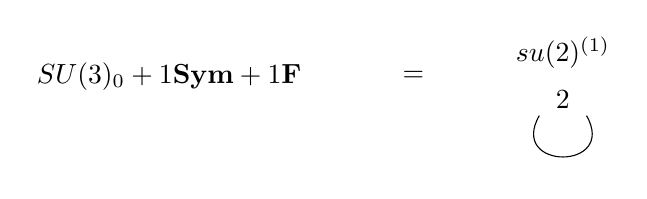
\begin{tikzpicture}
\draw (0, 0) node {$ SU(3)_0 + 1\mathbf{Sym} + 1\mathbf{F} $}
(3.1, 0) node {$ = $}
(5, 0.3) node {$ \mathfrak{su}(2)^{(1)} $}
(5, -0.3) node {$ 2 $}
;
\draw (4.7, -0.5) .. controls (4.3, -1.2) and (5.7, -1.2) .. (5.3, -0.5);
\end{tikzpicture}
\end{align}
This is another non-geometric rank-2 theory that can be realized by a brane web with $O7^+$ plane. The associated brane web will be given in Appendix~\ref{sec:appendix2}.

We can compute the BPS spectrum of this theory using the blowup formula.
The effective prepotential of this theory on the chamber $\phi_2\ge\phi_1>0$  is given by
\begin{align}
\mathcal{E} & = \frac{1}{\epsilon_1 \epsilon_2} \bigg( \mathcal{F} - \frac{\epsilon_1^2 + \epsilon_2^2}{48} (4\phi_1 - 4\phi_2) + \Big(\frac{\epsilon_1 + \epsilon_2}{2}\Big)^2 (\phi_1 + \phi_2)\bigg) \,, \nonumber \\
6\mathcal{F}
&= 8\phi_1^3 - 3\phi_1^2 \phi_2 - 3\phi_1 \phi_2^2 + 8\phi_2^3 + 6m_0(\phi_1^2 - \phi_1 \phi_2 + \phi_2^2) \nonumber \\
& \quad - \frac{1}{2} \big((2\phi_1\! + \!m_1)^3 + (\phi_2 \!+\! m_1)^3 + (-2\phi_1 \!+\! 2\phi_2 + m_1)^3 + (-\phi_1 \!+\! \phi_2 - m_1)^3 + (\phi_1 \!-\! m_1)^3\big) \nonumber \\
& \quad - \frac{1}{2} \big( (\phi_1 + m_2)^3 + (-\phi_1 + \phi_2 + m_2)^3 + (\phi_2 - m_2)^3 \big),
\end{align}
where $ m_0 $ is the gauge coupling, $ m_1 $ and $ m_2 $ are mass parameters of the symmetric and fundamental hypers, respectively. 
One finds a set of consistent magnetic fluxes
\begin{align}
n_i \in \mathbb{Z} \, , \quad
B_{m_0} = 0 \, , \quad
B_{m_1} = 1/2 \, , \quad
B_{m_2} = 1/2 \ ,
\end{align}
which provides a solvable unity blowup equation. The BPS spectrum from the solution of the blowup equation is given in Table~\ref{table:SU3_sym_F}.
\begin{table}
	\centering
	\begin{tabular}{|c|C{19ex}||c|C{19ex}|} \hline
		$ \mathbf{d} $ & $ \oplus N_{j_l, j_r}^{\mathbf{d}} (j_l, j_r) $ & $ \mathbf{d} $ & $ \oplus N_{j_l, j_r}^{\mathbf{d}} (j_l, j_r) $ \\ \hline
		$ (1, -\frac{2}{3}, \frac{2}{3}, \frac{3}{2}, \frac{1}{2}) $ & $ (0, \frac{1}{2}) $ & $ (1, -\frac{1}{3}, \frac{1}{3}, \frac{3}{2}, -\frac{1}{2}) $ & $ (0, 0) $ \\ \hline
		$ (1, -\frac{1}{3}, \frac{1}{3}, \frac{5}{2}, \frac{1}{2}) $ & $ (0, 0) $ & $ (1, 0, 1, \frac{1}{2}, \frac{1}{2}) $ & $ \! (0, 0) \oplus (0, 1) \oplus (\frac{1}{2}, \frac{1}{2}) \! $ \\ \hline
		$ (1, 0, 1, \frac{5}{2}, -\frac{1}{2}) $ & $ (0, \frac{1}{2}) $ & $ (1, \frac{1}{3}, -\frac{1}{3}, -\frac{5}{2}, -\frac{1}{2}) $ & $ (0, 0) $ \\ \hline
		$ (1, \frac{1}{3}, -\frac{1}{3}, -\frac{3}{2}, \frac{1}{2}) $ & $ (0, 0) $ & $ (1, \frac{1}{3}, \frac{2}{3}, -\frac{5}{2}, -\frac{1}{2}) $ & $ (0, 0) $ \\ \hline
		$ (1, \frac{1}{3}, \frac{2}{3}, -\frac{3}{2}, \frac{1}{2}) $ & $ (0, 0) $ & $ (1, \frac{1}{3}, \frac{2}{3}, \frac{1}{2}, -\frac{1}{2}) $ & $ (0, \frac{1}{2}) \oplus (\frac{1}{2}, 0) $ \\ \hline
		$ (1, \frac{1}{3}, \frac{2}{3}, \frac{3}{2}, \frac{1}{2}) $ & $ 2(0, \frac{1}{2}) \oplus (\frac{1}{2}, 0) $ & $ (1, \frac{2}{3}, -\frac{2}{3}, -\frac{3}{2}, -\frac{1}{2}) $ & $ (0, \frac{1}{2}) $ \\ \hline
		$ (1, \frac{2}{3}, \frac{1}{3}, -\frac{3}{2}, -\frac{1}{2}) $ & $ 2(0, \frac{1}{2}) \oplus (\frac{1}{2}, 0) $ & $ (1, \frac{2}{3}, \frac{1}{3}, -\frac{1}{2}, \frac{1}{2}) $ & $ (0, \frac{1}{2}) \oplus (\frac{1}{2}, 0) $ \\ \hline
		$ (1, \frac{2}{3}, \frac{1}{3}, \frac{3}{2}, -\frac{1}{2}) $ & $ (0, 0) $ & $ (1, \frac{2}{3}, \frac{1}{3}, \frac{5}{2}, \frac{1}{2}) $ & $ (0, 0) $ \\ \hline
		$ (1, 1, 0, -\frac{5}{2}, \frac{1}{2}) $ & $ (0, \frac{1}{2}) $ & $ (1, 1, 0, -\frac{1}{2}, -\frac{1}{2}) $ & $ \! (0, 0) \oplus (0, 1) \oplus (\frac{1}{2}, \frac{1}{2}) \! $ \\ \hline
		$ (1, 1, 1, -\frac{5}{2}, \frac{1}{2}) $ & $ (0, \frac{1}{2}) $ & $ (1, 1, 1, -\frac{1}{2}, -\frac{1}{2}) $ & $ 3(0, 0) \oplus (0, 1) \oplus 2(\frac{1}{2}, \frac{1}{2}) $ \\ \hline
		$ (1, 1, 1, \frac{1}{2}, \frac{1}{2}) $ & $ 3(0, 0) \oplus (0, 1) \oplus 2(\frac{1}{2}, \frac{1}{2}) $ & $ (1, 1, 1, \frac{5}{2}, -\frac{1}{2}) $ & $ (0, \frac{1}{2}) $ \\ \hline
	\end{tabular}
	\caption{BPS spectrum of the $SU(3)_0 + 1\mathbf{Sym} + 1\mathbf{F}$ theory. Here, $ \mathbf{d} = (d_1, d_2, d_3, d_4, d_5) $ labels the BPS states with charge $ d_1 m_0 + d_2 \alpha_1 + d_3 \alpha_2 + d_4 m_1 + d_5 m_2 $ where $ \alpha_1 $ and $ \alpha_2 $ are simple roots of $ \mathfrak{su}(3) $. } \label{table:SU3_sym_F}
\end{table}


\subsubsection{\texorpdfstring{$SU(3)_{\frac{15}{2}}+1\mathbf{F}$, $G_2+1\mathbf{Adj}$}{G2 + 1Adj}}

The last rank-2 KK theory is the theory obtained by $ \mathbb{Z}_3 $ twisted compactification of the 6d $\mathcal{N}=(2,0)$ $ D_4$ theory. This theory has two 5d gauge theory descriptions: one is the $G_2$ gauge theory with an adjoint hypermultiplet \cite{Tachikawa:2011ch} and another one is the $ SU(3)_{15/2} + 1\mathbf{F} $ theory \cite{Bhardwaj:2019jtr},
\begin{align}
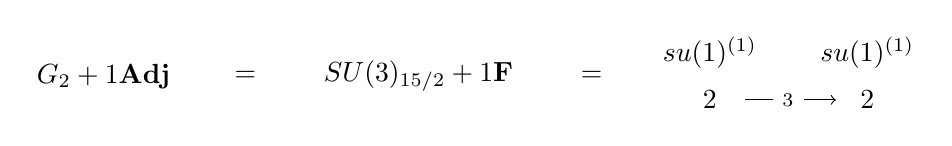
\begin{tikzpicture}
\draw (0, 0) node {$ G_2 + 1\mathbf{Adj} $}
(1.8, 0) node {$ = $}
(4, 0) node {$ SU(3)_{15/2} + 1\mathbf{F} $}
(6.2, 0) node {$ = $}
(7.7, 0.3) node {$ \mathfrak{su}(1)^{(1)} $}
(7.7, -0.3) node {$ 2 $}
(9.7, 0.3) node {$ \mathfrak{su}(1)^{(1)} $}
(9.7, -0.3) node {$ 2 $}
(8.15, -0.3) -- (8.5, -0.3)
(8.7, -0.3) node {$ _3 $}
;
\draw [->] (8.9, -0.3) -- (9.3, -0.3);
\end{tikzpicture}
\end{align}
It can be geometrically described by 
\begin{align}\label{eq:G2_adj_geo}
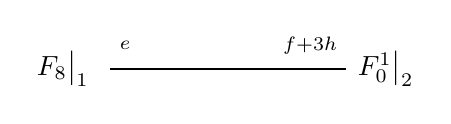
\begin{tikzpicture}
\draw[thick](-3,0)--(0,0);	
\node at(-3.6,0) {$\mathbb{F}_{8}{}\big|_1$};
\node at(-2.8,0.3) {${}_e$};
\node at(0.5,0) {$\mathbb{F}^1_{0}{}\big|_2$};
\node at(-0.45,0.3) {${}_{f+3h}$};
\end{tikzpicture} \ .
\end{align}
However, this geometry is not shrinkable and there is no known shrinkable geometric phase for this theory \cite{Jefferson:2018irk}. Nonetheless, it is expected that a series of flop transitions give rise to a phase for the unitary KK theory \cite{Bhardwaj:2019jtr}. As we will see below, this expectation is consistent with the BPS spectrum which we can compute by solving the blowup equations. 

We shall solve the blowup equations from both the $G_2$ and  $SU(3)$ theory perspectives. The effective prepotential for the $SU(3)$ theory on the Coulomb branch where $\phi_2\ge \phi_1>0$ is given by
\begin{align}
\mathcal{E} &= \frac{1}{\epsilon_1 \epsilon_2} \qty(\mathcal{F} - \frac{\epsilon_1^2 + \epsilon_2^2}{48} \big(4\phi_1 + 2\phi_2\big) + \epsilon_+^2 \qty(\phi_1 + \phi_2) ) \,, \nonumber \\
6\mathcal{F}
&= 8\phi_1^3 - 3\phi_1^2 \phi_2 - 3\phi_1 \phi_2^2 + 8\phi_2^3 + \frac{45}{2} \phi_1 \phi_2(\phi_1 - \phi_2) + 6m_0 (\phi_1^2 - \phi_1 \phi_2 + \phi_2^2) \nonumber \\
& \quad - \frac{1}{2} \Big((\phi_2 - m_1)^3 + (\phi_2 - \phi_1 + m_1)^3 + (\phi_1 + m_1)^3\Big) \,,
\end{align}
where $m_0$ is the $SU(3)$ gauge coupling and $m_1$ is the mass parameter of the fundamental hyper.

In the $G_2$ gauge theory, the effective prepotential in the same chamber is
\begin{align}
\mathcal{E} &= \frac{1}{\epsilon_1 \epsilon_2} \bigg( \mathcal{F} - \frac{\epsilon_1^2 + \epsilon_2^2}{48} (4\phi_1 + 2\phi_2) + \epsilon_+^2 (\phi_1 + \phi_2)\bigg) \,, \nonumber \\
6\mathcal{F}
&= 8\phi_1^3 + 18\phi_1^2 \phi_2 - 24\phi_1 \phi_2^2 + 8\phi_2^3 + 6m_0 (3\phi_1^2 - 3\phi_1 \phi_2 + \phi_2^2) \nonumber \\
& \quad -\frac{1}{2} \big((\phi_2 \pm m_1)^3 + (\pm(3\phi_1 - \phi_2) + m_1)^3 + (\pm \phi_1 + m_1)^3 + (\pm(\phi_2 - \phi_1) + m_1)^3 \nonumber \\
& \qquad \qquad + (\pm(-3\phi_1 + 2\phi_2) + m_1)^3 + (\pm(2\phi_1 - \phi_2) + m_1)^3) \big),
\end{align}
where $m_0$ is the $G_2$ gauge coupling and $m_1$ is the mass parameter of the adjoint matter. 

Under the duality, the K\"ahler parameters in the $ G_2 + 1\mathbf{Adj} $ and in the $ SU(3)_{15/2} + 1\mathbf{F} $ theories are mapped to each other as follows:
\begin{align}\label{eq:G2adj-su3+1f_map}
\phi_1^{G_2} &= \phi_1^{SU} + m_0^{SU} - \frac{1}{2} m_1^{SU} \,, \ \ \phi_2^{G_2} = \phi_2^{SU} + 2m_0^{SU(3)} - m_1^{SU} \,, \cr 
m_0^{G_2} &= 5m_0^{SU} + \frac{3}{2}m_1^{SU} \,, \ \ m_1^{G_2} = 2m_0^{SU}.
\end{align}
One can check with this map that the effective prepotentials of two dual gauge theories match well up to constant terms.

We first solve the blowup equation from the perspective of $ G_2 $ gauge theory. A set of consistent magnetic fluxes 
\begin{align}\label{eq:G2_adj_flux}
n_i \in \mathbb{Z} \, , \quad
B_{m_0} = 0 \, , \quad
B_{m_1} = 1/2 \ 
\end{align}
provides a solvable blowup equation.
By solving the blowup equation, we find the BPS spectrum of the $G_2$ gauge theory given in Table~\ref{table:G2_adj}.

\begin{table}
	\centering
	\begin{tabular}{|c|C{26ex}||c|C{26ex}|} \hline
		$ \mathbf{d} $ & $ \oplus N_{j_l, j_r}^{\mathbf{d}} (j_l, j_r) $ & $ \mathbf{d}$ & $\oplus N_{j_l, j_r}^{\mathbf{d}} (j_l, j_r) $ \\ \hline
		$ (1, 0, 1, 0) $ & $ 2(0,\frac{1}{2}) \oplus (\frac{1}{2},0) \oplus (\frac{1}{2},1) $ & $ (1, 0, 1, 1) $ & $ (0,0) \oplus (0,1) \oplus (\frac{1}{2},\frac{1}{2}) $ \\ \hline
		$ (1, 0, 1, 2) $ & $ (0, \frac{1}{2}) $ & $ (1, 0, 2, 0) $ & $ 2(0,\frac{3}{2}) \oplus (\frac{1}{2},1) \oplus (\frac{1}{2},2) $ \\ \hline
		$ (1, 0, 2, 1) $ & $ (0,1) \oplus (0,2) \oplus (\frac{1}{2},\frac{3}{2}) $ & $ (1, 0, 2, 2) $ & $ (0, \frac{3}{2}) $ \\ \hline
		$ (1, 1, 1, 0) $ & $ 4(0,\frac{1}{2}) \oplus 3(\frac{1}{2},0) \oplus (\frac{1}{2},1) $ & $ (1, 1, 1, 1) $ & $ 4(0,0) \oplus (0,1) \oplus 2(\frac{1}{2},\frac{1}{2}) $ \\ \hline
		$ (1, 1, 1, 2) $ & $ 2(0,\frac{1}{2}) \oplus (\frac{1}{2},0) $ & $ (1, 1, 1, 3) $ & $ (0, 0) $  \\ \hline
		$ (1, 1, 2, 0) $ & $ 4(0,\frac{1}{2}) \oplus 4(0,\frac{3}{2}) \oplus (\frac{1}{2},0) \oplus 4(\frac{1}{2},1) \oplus (\frac{1}{2},2) $ & $ (1, 1, 2, 1) $ & $ (0,0) \oplus 5(0,1) \oplus (0,2) \oplus 2(\frac{1}{2},\frac{1}{2}) \oplus 2(\frac{1}{2},\frac{3}{2}) $ \\ \hline
		$ (1, 1, 2, 2) $ & $ 2(0,\frac{1}{2}) \oplus 2(0,\frac{3}{2}) \oplus (\frac{1}{2},1) $ & $ (1, 1, 2, 3) $ & $ (0, 1) $ \\ \hline
		$ (1, 2, 1, 0) $ & $ 4(0,\frac{1}{2}) \oplus 3(\frac{1}{2},0) \oplus (\frac{1}{2},1) $ & $ (1, 2, 1, 1) $ & $ 4(0,0) \oplus (0,1) \oplus 2(\frac{1}{2},\frac{1}{2}) $ \\ \hline
		$ (1, 2, 1, 2) $ & $ 2(0,\frac{1}{2}) \oplus (\frac{1}{2},0) $ & $ (1, 2, 1, 3) $ & $ (0, 0) $  \\ \hline
		$ (1, 2, 2, 0) $ & $ 8(0,\frac{1}{2}) \oplus 4(0,\frac{3}{2}) \oplus 4(\frac{1}{2},0) \oplus 5(\frac{1}{2},1) \oplus (\frac{1}{2},2) $ & $ (1, 2, 2, 1) $ & $ 5(0,0) \oplus 6(0,1) \oplus (0,2) \oplus 4(\frac{1}{2},\frac{1}{2}) \oplus 2(\frac{1}{2},\frac{3}{2}) $ \\ \hline
		$ (1, 2, 2, 2) $ & $ 4(0,\frac{1}{2}) \oplus 2(0,\frac{3}{2}) \oplus (\frac{1}{2},0) \oplus (\frac{1}{2},1) $ & $ (1, 2, 2, 3) $ & $ (0,0) \oplus (0,1) $ \\ \hline
		$ (2, 0, 1, 0) $ & $ 5(0,\frac{1}{2}) \oplus 1(0,\frac{3}{2}) \oplus 3(\frac{1}{2},0) \oplus 3(\frac{1}{2},1) \oplus (1,\frac{1}{2}) \oplus (1,\frac{3}{2}) $ & $ (2, 0, 1, 1) $ & $ 4(0,0) \oplus 2(0,1) \oplus 3(\frac{1}{2},\frac{1}{2}) \oplus (\frac{1}{2},\frac{3}{2}) \oplus (1,1) $ \\ \hline
		$ (2, 0, 1, 2) $ & $ 2(0,\frac{1}{2}) \oplus (\frac{1}{2},0) \oplus (\frac{1}{2},1) $ & $ (2, 0, 1, 3) $ & $ (0, 0) $ \\ \hline
		$ (2, 1, 1, 0) $ & $ \! 12(0,\frac{1}{2}) \oplus (0,\frac{3}{2}) \oplus 10(\frac{1}{2},0) \oplus 6(\frac{1}{2},1) \oplus 4(1,\frac{1}{2}) \oplus (1,\frac{3}{2}) \! $ & $ (2, 1, 1, 1) $ & $ \! 10(0,0) \oplus 4(0,1) \oplus 9(\frac{1}{2},\frac{1}{2}) \oplus (\frac{1}{2},\frac{3}{2}) \oplus 2(1,0) \oplus 2(1,1) \! $ \\ \hline
		$ (2, 1, 1, 2) $ & $ 5(0,\frac{1}{2}) \oplus 4(\frac{1}{2},0) \oplus 2(\frac{1}{2},1) \oplus (1,\frac{1}{2}) $ & $ (2, 1, 1, 3) $ & $ 2(0,0) \oplus (\frac{1}{2},\frac{1}{2}) $ \\ \hline
	\end{tabular}
	\caption{BPS spectrum of the $ G_2 + 1\mathbf{Adj} $ for $ d_1 = 1 $, $ d_2, d_3 \leq 2 $ and $ d_1 = 2 $, $ d_2, d_3 \leq 1 $. Here, $ \mathbf{d} = (d_1, d_2, d_3, d_4) $ labels the BPS states with charge $ d_1 m_0 + d_2 \alpha_1 + d_3 \alpha_2 + d_4 m_1 $, where $ \alpha_1 = 2\phi_1 - \phi_2 $ and $ \alpha_2 = -3\phi_1 + 2\phi_2 $ are simple roots of $ G_2 $. The theory has a symmetry exchanging $ d_4 \leftrightarrow -d_4 $.} \label{table:G2_adj}
\end{table}

In the $ SU(3) $ description, one can use the same magnetic fluxes to formulate a unity blowup equation. The duality map \eqref{eq:G2adj-su3+1f_map} implies that the above fluxes in the $G_2$ perspective are converted into the magnetic fluxes in the $SU(3)$ gauge theory given by 
\begin{align}
n_1 \in \mathbb{Z} + 1/3 \, , \quad
n_2 \in \mathbb{Z} + 2/3 \, , \quad
B_{m_0} = 1/4 \, , \quad
B_{m_1} = -5/6 \ .
\end{align}
We checked that the blowup equation with these fluxes in the $SU(3)$ perspective can be solved and the solution perfectly agrees with the result from the $ G_2 + 1\mathbf{Adj} $ description.

The BPS spectrum tells us how to move on to the unitary phase where all the BPS states have non-negative masses in the UV limit. First note that the geometric phase \eqref{eq:G2_adj_geo} is non-shrinkable due to an exceptional curve $f_2-x$ whose volume cannot be non-negative while keeping volumes of all other curves non-negative at the same time. This implies that we need to flop the $f_2-x$ curve in the UV limit. Unfortunately, this transition leads to a phase which cannot be described by a smooth CY 3-fold.

However, we are able to trace all the phase transitions toward the unitary phase relying on the BPS spectrum we computed. To move on  to the unitary phase, we need to  flop 4 curves associated with 4 hypermultiplets with the masses, consecutively as,
\begin{equation}
	m_1-3\phi_1+\phi_2 \ \ \rightarrow \ \ m_1 -\phi_1 \ \  \rightarrow \ \ m_1 + \phi_1-\phi_2 \ \ \rightarrow \ \ m_1 +3\phi_1-2\phi_2 
\end{equation}
in the $G_2$ description. In the $SU(3)$ description, these hypermultiplets are all instantonic states. In the geometry \eqref{eq:G2_adj_geo}, the flop transitions performed on the exceptional curves as
\begin{equation}\label{eq:G2-flop}
	f_2 -x \ \ \rightarrow \ \ f_1+f_2 -x \ \ \rightarrow \ \ 2f_1+f_2 -x \ \rightarrow \ \ 3f_1+f_2 -x \ ,
\end{equation}
will lead to the unitary phase smoothly connected to the UV fixed point. One can check that in the final phase all the BPS states have non-negative masses. This result provides a strong evidence that the flop transitions in \eqref{eq:G2-flop} in the geometric description \eqref{eq:G2_adj_geo} are physically well-established transitions, though the phases after the flop transitions are non-geometrical.


\subsection{Rank 2 5d SCFTs}\label{sec:rank2SCFTs}

\subsubsection{\texorpdfstring{$ \mathbb{P}^2 \cup \mathbb{F}_3 $}{P2 U F3}}

The local $\mathbb{P}^2 \cup \mathbb{F}_3 $ theory is a rank-2 analog of the SCFT engineered by a local $\mathbb{P}^2$. It is a non-Lagrangian theory with no mass parameter. Its geometric construction is represented by
\begin{align}
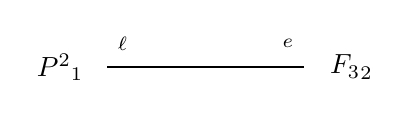
\begin{tikzpicture}
\draw[thick](-2.5,0)--(0,0);	
\node at(-3.1,0) {$\eval{\mathbb{P}^2}_1$};
\node at(-2.3,0.3) {${}_\ell$};
\node at(0.6,0) {$\eval{\mathbb{F}_{3}}_2$};
\node at(-0.2,0.3) {${}_{e}$};
\end{tikzpicture} \ .
\end{align}
The volumes of two primitive 2-cycles are given by
\begin{align}
\vol(\ell) = 3\phi_1 - \phi_2 \ , \quad
\vol(f_2) = -\phi_1 + 2\phi_2\ ,
\end{align}
where $\ell$ is a curve with $\ell^2=1$ in $\mathbb{P}^2$ and $ f_2 $ is the fiber in $ \mathbb{F}_3 $. The geometry can be obtained by blowing down an exceptional cycle of $ \mathbb{F}_1 $ in geometry $ \mathbb{F}_1 - \mathbb{F}_3 $, which implies that this theory can be obtained by an RG flow from  the pure $ SU(3)_2 $ theory by integrating out an instantonic hypermultiplet. The web diagram for this theory is depicted in Figure~\ref{fig:P2-F3}.
\begin{figure}
	\centering
	\begin{subfigure}[b]{0.33\textwidth}
		\centering
		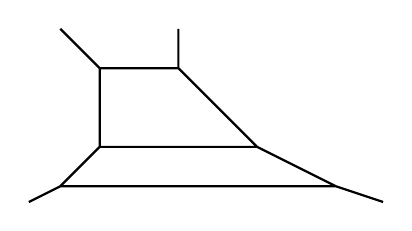
\begin{tikzpicture}
		\draw[thick] (0.5, 0.5) -- (1, 1) -- (1, 2) -- (2, 2) -- (3, 1) -- (1, 1)
		(1, 2) -- (0.5, 2.5)
		(2, 2) -- (2, 2.5)
		(3, 1) -- (4, 0.5)
		(0.1, 0.3) -- (0.5, 0.5) -- (4, 0.5) -- (4.6, 0.3);
		\end{tikzpicture}
		\caption{}
	\end{subfigure}
	\begin{subfigure}[b]{0.31\textwidth}
		\centering
		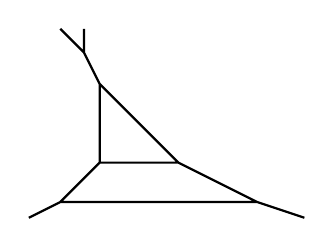
\begin{tikzpicture}
		\draw[thick] (0.5, 0.5) -- (1, 1) -- (1, 2) -- (2, 1) -- (1, 1)
		(1, 2) -- (0.8, 2.4) -- (0.8, 2.7)
		(0.8, 2.4) -- (0.5, 2.7)
		(2, 1) -- (3, 0.5)
		(0.1, 0.3) -- (0.5, 0.5) -- (3, 0.5) -- (3.6, 0.3);
		\end{tikzpicture}
		\caption{}
	\end{subfigure}
	\begin{subfigure}[b]{0.32\textwidth}
		\centering
		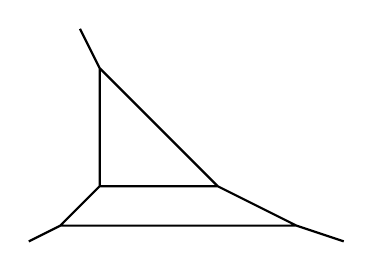
\begin{tikzpicture}
		\draw[thick] (0.5, 0.5) -- (1, 1) -- (1, 2.5) -- (2.5, 1) -- (1, 1)
		(1, 2.5) -- (0.75, 3)
		(2.5, 1) -- (3.5, 0.5)
		(0.1, 0.3) -- (0.5, 0.5) -- (3.5, 0.5) -- (4.1, 0.3);
		\end{tikzpicture}
		\caption{}
	\end{subfigure}
	\caption{A 5-brane web construction for $ \mathbb{P}^2 \cup \mathbb{F}_3 $. Starting from the web diagram of $ SU(3)_2 $ theory (a), flop transition for an instantonic hypermultiplet gives (b). Integrating out the hypermultiplet gives a web diagram of $ \mathbb{P}^2 \cup \mathbb{F}_3 $ depicted in (c).} \label{fig:P2-F3}
\end{figure}

The effective prepotential on the $\Omega$-background is
\begin{align}
\mathcal{E} &= \frac{1}{\epsilon_1 \epsilon_2} \qty(\mathcal{F} - \frac{\epsilon_1^2 + \epsilon_2^2}{48}(6\phi_1 + 4\phi_2) + \epsilon_+^2 (\phi_1 + \phi_2)) \ , \nonumber \\
6\mathcal{F} &= 9\phi_1^3 - 9\phi_1^2 \phi_2 + 3\phi_1 \phi_2^2 + 8\phi_2^3 \ .
\end{align}
For a unity blowup equation, we choose the magnetic fluxes as
\begin{align}
n_1 \in \mathbb{Z} + 1/5 \ , \quad
n_2 \in \mathbb{Z} + 1/10 \ ,
\end{align}
which assign half-integral fluxes for $ \ell $ and integral fluxes for $ f_2 $. The BPS spectrum obtained by solving the blowup equation is given in Table~\ref{table:P2-F3}. We checked that the result matches the spectrum after taking an RG flow from the BPS spectrum of the pure $ SU(3)_2 $ theory by integrating out the instantonic hypermultiplet.

\begin{table}
	\centering
	\begin{tabular}{|c|C{29ex}||c|C{29ex}|} \hline
		$\mathbf{d}$ & $\oplus N_{j_l, j_r}^{\mathbf{d}} (j_l, j_r)$ & $\mathbf{d}$ & $\oplus N_{j_l, j_r}^{\mathbf{d}} (j_l, j_r)$ \\ \hline
		$ (0, 1) $ & $ (0, \frac{1}{2}) $ & $ (1, 0) $ & $ (0, 1) $ \\ \hline
		$ (1, 1) $ & $ (0, 0) \oplus (0, 1) $ & $ (1, 2) $ & $ (0, 1) $ \\ \hline
		$ (1, 3) $ & $ (0, 2) $ & $ (2, 0) $ & $ (0, \frac{5}{2}) $ \\ \hline
		$ (2, 1) $ & $ (0, \frac{3}{2}) \oplus (0, \frac{5}{2}) $ & $ (2, 2) $ & $ (0, \frac{1}{2}) \oplus (0, \frac{3}{2}) \oplus (0, \frac{5}{2}) $ \\ \hline
		$ (2, 3) $ & $ (0, \frac{1}{2}) \oplus (0, \frac{3}{2}) \oplus (0, \frac{5}{2}) $ & $ (3, 0) $ & $ (0, 3) \oplus (\frac{1}{2}, \frac{9}{2}) $ \\ \hline
		$ (3, 1) $ & $ (0,2) \oplus 2(0,3) \oplus (0,4) \oplus (\frac{1}{2},\frac{7}{2}) \oplus (\frac{1}{2},\frac{9}{2}) $ & $ (3, 2) $ & $ (0,1) \oplus 2(0,2) \oplus 3(0,3) \oplus (0,4) \oplus (\frac{1}{2},\frac{5}{2}) \oplus (\frac{1}{2},\frac{7}{2}) \oplus (\frac{1}{2},\frac{9}{2}) $ \\ \hline
		$ (3, 3) $ & \multicolumn{3}{C{67ex}|}{$ \! (0,0) \oplus 2(0,1) \oplus 3(0,2) \oplus 3(0,3) \oplus (0,4) \oplus (\frac{1}{2},\frac{3}{2}) \oplus (\frac{1}{2},\frac{5}{2}) \oplus (\frac{1}{2},\frac{7}{2}) \oplus (\frac{1}{2},\frac{9}{2}) \! $} \\ \hline
	\end{tabular}
	\caption{BPS spectrum of $ \mathbb{P}^2 \cup \mathbb{F}_3 $ for $ d_i \leq 3 $. Here, $ \mathbf{d} = (d_1, d_2) $ labels the BPS states with charge $ d_1 \ell + d_2 f_2 $.}\label{table:P2-F3}
\end{table}


\subsubsection{\texorpdfstring{$ \mathbb{P}^2 \cup \mathbb{F}_6 $}{P2 U F6}}

The local $ \mathbb{P}^2 \cup \mathbb{F}_6 $ theory is another non-Lagrangian rank-2 theory with no mass parameter. Its geometric construction is given by
\begin{align}
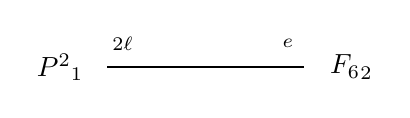
\begin{tikzpicture}
\draw[thick](-2.5,0)--(0,0);	
\node at(-3.1,0) {$\eval{\mathbb{P}^2}_1$};
\node at(-2.3,0.3) {${}_{2\ell}$};
\node at(0.6,0) {$\eval{\mathbb{F}_{6}}_2$};
\node at(-0.2,0.3) {${}_{e}$};
\end{tikzpicture} \ .
\end{align}
The volumes of two primitive 2-cycles are
\begin{align}
\vol(\ell) = 3\phi_1 - 2\phi_2 \, , \quad
\vol(f_2) = -\phi_1 + 2\phi_2
\end{align}
where $ \ell $ is the curve class in $ \mathbb{P}^2 $ and $ f_2 $ is the fiber in $ \mathbb{F}_6 $. This theory can be obtained by an integrating out an instantonic hypermultiplet of the pure $ SU(3)_4 $ theory. The web diagram and the RG flow of this theory are given in Figure~\ref{fig:P2-F6}.
\begin{figure}
	\centering
	\begin{subfigure}[b]{0.32\textwidth}
		\centering
		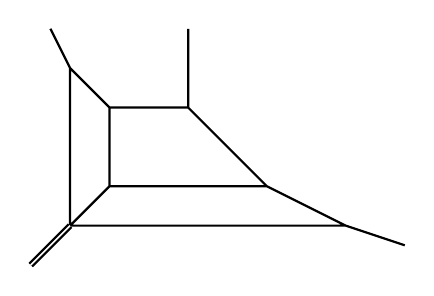
\begin{tikzpicture}
		\draw[thick] (0.5, 0.5) -- (1, 1) -- (1, 2) -- (2, 2) -- (3, 1)
		(1, 1) -- (3, 1)
		(1, 2) -- (0.5, 2.5) -- (0.5, 0.5) -- (4, 0.5) -- (3, 1)
		(0.5, 2.5) -- (0.25, 3)
		(2, 2) -- (2, 3)
		(4, 0.5) -- (4.75, 0.25);
		\draw[thick, double] (0, 0) -- (0.5, 0.5);
		\end{tikzpicture}
		\caption{}
	\end{subfigure}
	\begin{subfigure}[b]{0.32\textwidth}
		\centering
		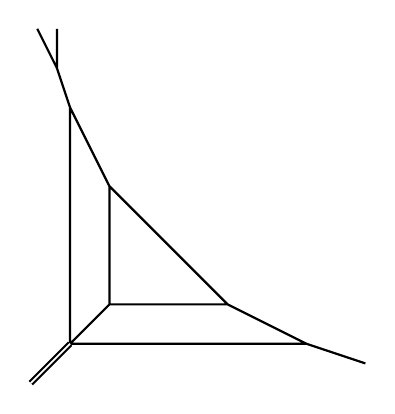
\begin{tikzpicture}
		\draw[thick] (0.5, 0.5) -- (1, 1) -- (1, 2.5) -- (2.5, 1) -- (3.5, 0.5) -- (4.25, 0.25)
		(1, 1) -- (2.5, 1)
		(3.5, 0.5) -- (0.5, 0.5) -- (0.5, 3.5) -- (1, 2.5)
		(0.5, 3.5) -- (0.333, 4) -- (0.333, 4.5)
		(0.333, 4) -- (0.083, 4.5);
		\draw[thick, double] (0, 0) -- (0.5, 0.5);
		\end{tikzpicture}
		\caption{}
	\end{subfigure}
	\begin{subfigure}[b]{0.32\textwidth}
		\centering
		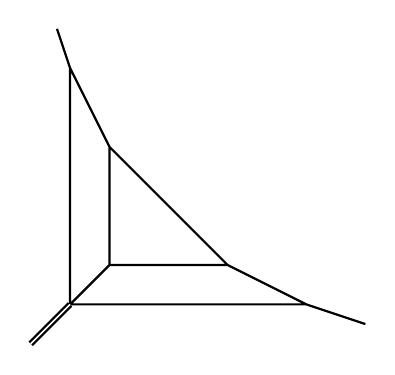
\begin{tikzpicture}
		\draw[thick] (0.5, 0.5) -- (1, 1) -- (1, 2.5) -- (2.5, 1) -- (3.5, 0.5) -- (4.25, 0.25)
		(1, 1) -- (2.5, 1)
		(3.5, 0.5) -- (0.5, 0.5) -- (0.5, 3.5) -- (1, 2.5)
		(0.5, 3.5) -- (0.333, 4);
		\draw[thick, double] (0, 0) -- (0.5, 0.5);
		\end{tikzpicture}
		\caption{}
	\end{subfigure}
	\caption{A 5-brane web construction for $ \mathbb{P}^2 \cup \mathbb{F}_6 $. Starting from the web diagram of $ SU(3)_4 $ theory (a), flop transition of two instantonic hypermultiplets gives (b). Integrating out the hypermultiplet gives a web diagram of $ \mathbb{P}^2 \cup \mathbb{F}_6 $ depicted in (c).} \label{fig:P2-F6}
\end{figure}

The effective prepotential is
\begin{align}
\mathcal{E} &= \frac{1}{\epsilon_1 \epsilon_2} \qty( \mathcal{F} - \frac{\epsilon_1^2 + \epsilon_2^2}{48}(6\phi_1 + 4\phi_2) + \epsilon_+^2 (\phi_1 + \phi_2) ) \, ,  \nonumber \\
6\mathcal{F} &= 9\phi_1^3 - 18\phi_1^2 \phi_2 + 12\phi_1 \phi_2^2 + 8\phi_2^3 \ .
\end{align}
We choose the magnetic fluxes
\begin{align}
n_1 \in \mathbb{Z} + 1/4 \, , \quad
n_2 \in \mathbb{Z} + 1/8\ ,
\end{align}
to get a solvable unity blowup equation. The BPS spectrum obtained by solving the blowup equation is given in Table~\ref{table:P2-F6}.  We checked that the result matches the spectrum after taking an RG flow from the BPS spectrum of the pure $ SU(3)_4 $ theory given in Table \ref{table:SU(3)_4} by integrating out the instantonic hypermultiplet.

\begin{table}
	\centering
	\begin{tabular}{|c|C{29ex}||c|C{29ex}|} \hline
		$\mathbf{d}$ & $\oplus N_{j_l, j_r}^{\mathbf{d}} (j_l, j_r)$ & $\mathbf{d}$ & $\oplus N_{j_l, j_r}^{\mathbf{d}} (j_l, j_r)$ \\ \hline
		$ (0, 1) $ & $ (0, \frac{1}{2}) $ & $ (1, 0) $ & $ (0, 1) $ \\ \hline
		$ (1, 1) $ & $ (0, 0) \oplus (0, 1) $ & $ (1, 2) $ & $ (0, 1) $ \\ \hline
		$ (2, 0) $ & $ (0, \frac{5}{2}) $ & $ (2, 1) $ & $ (0, \frac{3}{2}) \oplus (0, \frac{5}{2}) $ \\ \hline
		$ (2, 2) $ & $ (0,\frac{1}{2}) \oplus (0,\frac{3}{2}) \oplus (0,\frac{5}{2}) $ & $ (2, 3) $ & $ (0, \frac{1}{2}) \oplus (0, \frac{3}{2}) \oplus (0, \frac{5}{2}) $ \\ \hline
		$ (3, 0) $ & $ (0, 3) \oplus (\frac{1}{2}, \frac{9}{2}) $ & $ (3, 1) $ & $ (0,2) \oplus 2(0,3) \oplus (0,4) \oplus (\frac{1}{2},\frac{7}{2})\oplus (\frac{1}{2},\frac{9}{2}) $ \\ \hline
		$ (3, 2) $ & $ (0,1) \oplus 2(0,2) \oplus 3(0,3) \oplus (0,4) \oplus (\frac{1}{2},\frac{5}{2}) \oplus (\frac{1}{2},\frac{7}{2}) \oplus (\frac{1}{2},\frac{9}{2}) $ & $ (3, 3) $ & $ (0,0) \oplus 2(0,1) \oplus 3(0,2) \oplus 3(0,3) \oplus (0,4) \oplus (\frac{1}{2},\frac{3}{2}) \oplus (\frac{1}{2},\frac{5}{2}) \oplus (\frac{1}{2},\frac{7}{2}) \oplus (\frac{1}{2},\frac{9}{2}) $ \\ \hline
	\end{tabular}
	\caption{BPS spectrum of $ \mathbb{P}^2 \cup \mathbb{F}_6 $ for $ d_i \leq 3 $. Here, $ \mathbf{d} = (d_1, d_2) $ labels the BPS state with charge $ d_1 \ell + d_2 f_2 $.} \label{table:P2-F6}
\end{table}


\subsubsection{\texorpdfstring{$ \mathbb{P}^2 \cup \mathbb{F}_3 + 1\mathbf{Sym} $}{P2 U F3 + 1Sym}}

The $\mathbb{P}^2 \cup \mathbb{F}_3 + 1\mathbf{Sym}$ theory is a rank-2 analog of the local $\mathbb{P}^2+{\bf 1Adj}$ theory. As proposed in \cite{Bhardwaj:2019jtr}, we can obtain this theory from the UV $ Sp(2)_\pi + 1\mathbf{Adj} $ theory or $ SU(3)_{3/2} + 1\mathbf{Sym} $ theory by integrating out an instantonic hypermultiplet. See Appendix~\ref{sec:app-P2 U F3+1Sym} for their 5-brane constructions. 

More precisely, there is a hypermultiplet with $ \mathbf{d} = (1, \frac{2}{3}, \frac{1}{3}, -\frac{5}{2}) $ which has mass $ m_0 + \phi_1 - \frac{5}{2}m_1 $ in the UV parent theory, as listed in Table~\ref{table:SU3_1Sym}. We flop this hypermultiplet and integrate it out to get the $ \mathbb{P}^2 \cup \mathbb{F}_3 + 1\mathbf{Sym} $ theory in IR. This RG flow is realized in the 5-brane web in Figure~\ref{fig:P2-F3-Sym} as taking a limit $ -m_0 - \phi_1 + \frac{5}{2}m_1 \to \infty $ while the lengths of other edges are kept finite.
\begin{figure}
	\centering
	\begin{tikzpicture}
	\draw[thick] (0, 0) -- (3, 1) -- (5, 2) -- (6, 3) -- (6, 2) -- (7, 1) -- (9, 0)
	(5, 2) -- (6, 2)
	(3, 1) -- (7, 1)
	(6, 3) -- (6.5, 4) -- (6.5, 4.5)
	(6.5, 4) -- (7, 4.5)
	(11, 0) -- (10, 1);
	\draw[dashed] (-1, 0) -- (12, 0);
	\filldraw[fill=white, thick] (9, 0) circle (0.15);
	\draw (7.5, 3.5) node {\scriptsize{$ -m_0 - \phi_1 + \frac{5}{2}m_1 $}}
	(7.6, 2.5) node {\scriptsize{$ m_0 + 3\phi_1 - \phi_2 - \frac{5}{2}m_1 $}}
	(3, 1.7) node {\scriptsize{$ -\phi_1 + 2\phi_2 $}}
	(6.9, 0.4) node {\scriptsize{$ m_1 - 2\phi_2 $}}
	(9, -0.4) node {\scriptsize{$ O7^+ $}};
	\end{tikzpicture}
	\caption{A 5-brane web for $ SU(3)_{3/2} + 1\mathbf{Sym} $ and $Sp(2)_\pi + 1{\bf Adj}$, where a flop transition for the edge with length $\phi_1+m_0-\frac{5}{2}m_1$ is performed.} \label{fig:P2-F3-Sym}
\end{figure}

To compute the effective prepotential and the BPS partition function of this theory, it is convenient to redefine the parameters in the web diagram in Figure~\ref{fig:P2-F3-Sym} as
\begin{align}\label{eq:P2-F3_var_redef}
\tilde{\phi}_1 = \phi_1 + \frac{2}{5}m_0 - m_1 \, , \quad
\tilde{\phi}_2 = \phi_2 + \frac{m_0}{5} - \frac{m_1}{2} \, , \quad
\tilde{m} = \frac{2}{5} m_0 \ .
\end{align}
Then the volumes of 2-cycles in Figure~\ref{fig:P2-F3-Sym} become
\begin{align}
&-m_0 -\phi_1 + \frac{5}{2}m_1 = -\tilde{\phi}_1 - \frac{3}{2}\tilde{m} + \frac{3}{2}m_1 \, , \quad -\phi_1 + 2\phi_2 = -\tilde{\phi}_1 + 2\tilde{\phi}_2 \,,  \nonumber \\
&m_0 + 3\phi_1 - \phi_2 - \frac{5}{2}m_1 = 3\tilde{\phi}_1 - \tilde{\phi}_2 \, , \quad m_1 - 2\phi_2 = \tilde{m} - 2\tilde{\phi}_2 \ . 
\end{align}
Hence, the RG flow corresponds to the limit $ m_1 \to \infty $,  while keeping $ \tilde{\phi}_i $ and $ \tilde{m} $ finite.

The cubic prepotential and mixed gravitational Chern-Simons term in the IR $ \mathbb{P}^2 \cup \mathbb{F}_3 + 1\mathbf{Sym} $ theory can be obtained from those of the UV $ SU(3)_{3/2} + 1\mathbf{Sym} $ theory as follows:
\begin{align}
\mathcal{F}_{IR} = \mathcal{F}_{UV} + \frac{1}{6} \qty(m_0 + \phi_1 - \frac{5}{2}m_1)^3 \, , \quad
C_{IR} = C_{UV} - 2\qty(m_0 + \phi_1 - \frac{5}{2}m_1) \, ,
\end{align}
whereas the mixed gauge/$ SU(2)_R $ Chern-Simons term remains the same. In terms of the parameters in \eqref{eq:P2-F3_var_redef}, the effective prepotential in the IR theory takes the form
\begin{align}
\mathcal{E} &= \frac{1}{\epsilon_1 \epsilon_2} \qty(\mathcal{F}_{IR} - \frac{\epsilon_1^2 + \epsilon_2^2}{48} (6 \tilde{\phi}_1 + 4 \tilde{\phi}_2) + \epsilon_+^2 (\tilde{\phi}_1 + \tilde{\phi}_2) ) \, , \nonumber \\
6\mathcal{F}_{IR} &= 9\tilde{\phi}_1^3 - 9\tilde{\phi}_1^2 \tilde{\phi}_2 + 3\tilde{\phi}_1 \tilde{\phi}_2^2 + 8\tilde{\phi}_2^3 \ ,
\end{align}
up to constant terms. One may notice that the prepotential is the same as that of $ \mathbb{P}^2 \cup \mathbb{F}_3 $. However, this theory has an additional hypermultiplet coming from the symmetric matter of the parent theory. The GV-invariant for this hypermultiplet
\begin{align}
\mathcal{Z}_{\mathrm{hyper}}(\tilde{\phi}_i, \tilde{m}; \epsilon_{1,2})
= \PE\qty[ \frac{(p_1 p_2)^{1/2}}{(1-p_1)(1-p_2)} e^{-(\tilde{m} - 2\tilde{\phi}_2)}  ] 
\end{align}
is an additional input for the blowup equation of the IR theory.

We find a set of  consistent magnetic fluxes
\begin{align}
\tilde{n}_1 \in \mathbb{Z} - 3/5 \, , \quad
\tilde{n}_2 \in \mathbb{Z} - 3/10 \, , \quad
B_{\tilde{m}} = -1/10
\end{align}
which leads to a unity blowup equation. The solution of the blowup equation provides the BPS spectrum of the theory, summarized in Table~\ref{table:P2-F3+1Sym}. This solution matches the spectrum that we can obtain indirectly from the RG flow of the BPS spectrum in $ SU(3)_{3/2} + 1\mathbf{Sym} $ in Table~\ref{table:SU3_1Sym} after integrating out the hypermultiplet.

\begin{table}
	\centering
	\begin{tabular}{|c|C{28ex}||c|C{28ex}|} \hline
		$\mathbf{d}$ & $\oplus N_{j_l, j_r}^{\mathbf{d}} (j_l, j_r)$ & $\mathbf{d}$ & $\oplus N_{j_l, j_r}^{\mathbf{d}} (j_l, j_r)$ \\ \hline
		$ (1, 0, 0) $ & $ (0, 0) $ & $ (1, 0, 1) $ & $ (0, 0) $ \\ \hline
		$ (1, 0, 2) $ & $ (0, 0) $ & $ (1, 1, 1) $ & $ (0, \frac{1}{2}) $ \\ \hline
		$ (1, 1, 2) $ & $ 2(0, \frac{1}{2}) \oplus (\frac{1}{2}, 0) $ & $ (1, 1, 3) $ & $ (0, \frac{1}{2}) \oplus (0, \frac{3}{2}) \oplus (\frac{1}{2}, 1) $ \\ \hline
		$ (1, 2, 1) $ & $ (0, 2) $ & $ (1, 2, 2) $ & $ \! (0, 0) \oplus (0, 1) \oplus 2(0, 2) \oplus (\frac{1}{2}, \frac{3}{2}) \! $ \\ \hline
		$ (1, 2, 3) $ & $ 2(0,0) \oplus 3(0,1) \oplus 2(0,2) \oplus (\frac{1}{2},\frac{1}{2}) \oplus (\frac{1}{2},\frac{3}{2}) $ & $ (1, 3, 1) $ & $ (0,\frac{5}{2}) \oplus (0,\frac{7}{2}) \oplus (\frac{1}{2},4) $ \\ \hline
		$ (1, 3, 2) $ & $ 2(0,\frac{3}{2}) \oplus 4(0,\frac{5}{2}) \oplus 3(0,\frac{7}{2}) \oplus (\frac{1}{2},2) \oplus 2(\frac{1}{2},3) \oplus 2(\frac{1}{2},4) \oplus (1,\frac{7}{2}) $ & $ (1, 3, 3) $ & $ 2(0,\frac{1}{2}) \oplus 6(0,\frac{3}{2}) \oplus 8(0,\frac{5}{2}) \oplus 4(0,\frac{7}{2}) \oplus (\frac{1}{2},1) \oplus 4(\frac{1}{2},2) \oplus 4(\frac{1}{2},3) \oplus 2(\frac{1}{2},4) \oplus (1,\frac{5}{2}) \oplus (1,\frac{7}{2}) $ \\ \hline
		$ (2, 1, 3) $ & $ 2(0, 0) \oplus (\frac{1}{2}, \frac{1}{2}) $ & $ (2, 2, 3) $ & $ (0,\frac{1}{2}) \oplus (0,\frac{3}{2}) \oplus (\frac{1}{2},1) $ \\ \hline
		$ (2, 3, 2) $ & $ (0, 3) $ & $ (2, 3, 3) $ & $ (0,1) \oplus 3(0,2) \oplus 3(0,3) \oplus (\frac{1}{2},\frac{3}{2}) \oplus 2(\frac{1}{2},\frac{5}{2}) \oplus (\frac{1}{2},\frac{7}{2}) \oplus (1,3) $ \\ \hline
	\end{tabular}
	\caption{BPS spectrum of $ \mathbb{P}^2 \cup \mathbb{F}_3 + 1\mathbf{Sym} $ for $ d_1 \leq 2 $, $ d_2, d_3 \leq 3 $. Here, $ \mathbf{d} = (d_1, d_2, d_3) $ labels the BPS state with charge $ d_1(\tilde{m}-2\tilde{\phi}_2) + d_2(3\tilde{\phi}_1 - \tilde{\phi}_2) + d_3(-\tilde{\phi}_1 + 2\tilde{\phi}_2) $. The $ d_1 = 0 $ sector is the same with that of $ \mathbb{P}^2 \cup \mathbb{F}_3 $.} \label{table:P2-F3+1Sym}
\end{table}


\subsubsection{\texorpdfstring{$ \mathbb{P}^2 \cup \mathbb{F}_6 + 1\mathbf{Sym} $}{P2 U F6 + 1Sym}}

The theory $ \mathbb{P}^2 \cup \mathbb{F}_6 + 1\mathbf{Sym} $ is a non-Lagrangian theory obtained from the KK-theory $ SU(3)_0 + 1\mathbf{Sym} + 1\mathbf{F} $ by integrating out the fundamental hypermultiplet and an instantonic hypermultiplet together \cite{Bhardwaj:2019jtr}. The corresponding 5-brane web is given in Figure \ref{fig:P2-F6-Sym}. This theory can also be obtained from a non-perturbative Higgsing on  $SU(4)_0+1\mathbf{Sym}$. See Appendix~\ref{sec:app-P^2F_6+1Sym} for 5-brane construction and generalizations.

From $ SU(3)_0 + 1\mathbf{Sym} + 1\mathbf{F} $, we can first integrate out the fundamental matter. The IR theory then becomes the $ SU(3)_{-1/2} + 1\mathbf{Sym} $ theory, whose effective prepotential is given by
\begin{align}
\mathcal{E}_{SU(3)} & = \frac{1}{\epsilon_1 \epsilon_2} \qty( \mathcal{F}_{SU(3)} - \frac{\epsilon_1^2 + \epsilon_2^2}{24}(2\phi_1 + 2\phi_2 - 3m_1) + \epsilon_+^2 (\phi_1 + \phi_2))
 \,, \nonumber \\
6\mathcal{F}_{SU(3)}
&= 8\phi_1^3 - 3\phi_1^2 \phi_2 - 3\phi_1 \phi_2^2 + 8\phi_2^3 - \frac{3}{2} \phi_1 \phi_2 (\phi_1 - \phi_2) + 6m_0 (\phi_1^2 - \phi_1 \phi_2 + \phi_2^2) \nonumber \\
& \quad - \frac{1}{2} \Big( (2\phi_1 + m_1)^3 + (\phi_2 + m_1)^3 + (-2\phi_1 + 2\phi_2 + m_1)^3 \nonumber \\
& \qquad \quad + (\phi_1 - \phi_2 + m_1)^3 + (-\phi_1 + m_1)^3 + (-2\phi_1 + m_1)^3 \Big)\ ,
\end{align}
where $ m_0 $ is the gauge coupling and $ m_1 $ is the mass parameter of the symmetric matter. 

This theory has a set of consistent magnetic fluxes
\begin{align}
n_i \in \mathbb{Z} \, , \quad
B_{m_0} = -1/4 \, , \quad
B_{m_1} = 1/2 \ ,
\end{align}
which gives a unity blowup equation. Solving the blowup equation yields the BPS spectrum of this theory.

Among the BPS states in $ SU(3)_{-1/2} + 1\mathbf{Sym} $ theory, there are instantonic hypermultiplets whose masses are $ m_0 + \phi_1 - \phi_2 - \frac{5}{2}m_1 $ and $ m_0 + \phi_2 - \frac{5}{2}m_1 $. In terms of $ SU(3)_0 + 1\mathbf{Sym} + 1\mathbf{F} $ theory given in Table~\ref{table:SU3_sym_F}, they correspond to $ \mathbf{d} = (1, \frac{1}{3}, -\frac{1}{3}, -\frac{5}{2}, -\frac{1}{2}) $ and $ \mathbf{d} = (1, \frac{1}{3}, \frac{2}{3}, -\frac{5}{2}, -\frac{1}{2}) $, respectively. We can perform flop transitions for these two hypermultiplets to get a 5-brane web shown in Figure~\ref{fig:P2-F6-Sym}.

\begin{figure}
	\centering
	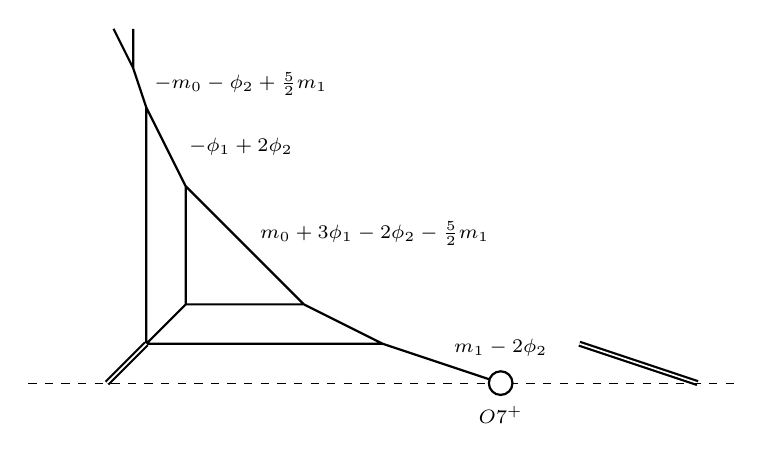
\begin{tikzpicture}
	\draw[thick] (0.5, 0.5) -- (1, 1) -- (1, 2.5) -- (2.5, 1) -- (3.5, 0.5) -- (5, 0)
	(1, 1) -- (2.5, 1)
	(3.5, 0.5) -- (0.5, 0.5) -- (0.5, 3.5) -- (1, 2.5)
	(0.5, 3.5) -- (0.333, 4) -- (0.333, 4.5)
	(0.333, 4) -- (0.083, 4.5);
	\draw[thick, double] (0, 0) -- (0.5, 0.5)
	(7.5, 0) -- (6, 0.5);
	\draw[dashed] (-1, 0) -- (8, 0);
	\filldraw[fill=white, thick] (5, 0) circle (0.15);
	\draw (5, -0.4) node {\scriptsize{$ O7^+ $}}
	(1.7, 3.8) node {\scriptsize{$ -m_0 - \phi_2 + \frac{5}{2}m_1 $}}
	(1.7, 3) node {\scriptsize{$ -\phi_1 + 2\phi_2 $}}
	(3.4, 1.9) node {\scriptsize{$ m_0 + 3\phi_1 - 2\phi_2 - \frac{5}{2}m_1 $}}
	(5, 0.45) node {\scriptsize{$ m_1 - 2\phi_2 $}};
	\end{tikzpicture}
	\caption{A 5-brane web for $ SU(3)_{-1/2} + 1\mathbf{Sym} $, after flopping the edges with lengths $ m_0 + \phi_1 - \phi_2 - \frac{5}{2}m_1 $ and $ m_0 + \phi_2 -\frac{5}{2}m_1 $.} \label{fig:P2-F6-Sym}
\end{figure}

The $ SU(3)_{-1/2} + 1\mathbf{Sym} $ theory has an RG flow to the $ \mathbb{P}^2 \cup \mathbb{F}_6 + 1\mathbf{Sym} $ theory. The RG flow is generated by integrating out the instantonic hypermultiplet corresponding to the limit $ -m_0 - \phi_2 + \frac{5}{2}m_1 \to \infty $, while keeping the lengths of other edges finite, in the brane web. To see this, it is convenient to use the parameters as
\begin{align}\label{eq:P2-F6-var-redef}
\tilde{\phi}_1 = \phi_1 + \frac{m_0}{2} - \frac{5}{4}m_1 \, , \quad
\tilde{\phi}_2 = \phi_2 + \frac{m_0}{4} - \frac{5}{8}m_1 \, , \quad
\tilde{m} = \frac{m_0}{2} - \frac{m_1}{4} \ .
\end{align}
Then volumes of 2-cycles in Figure~\ref{fig:P2-F6-Sym} become
\begin{align}
&-m_0 - \phi_2 + \frac{5}{2}m_1 = -\tilde{\phi}_2 + 3m_0 - \frac{15}{2}\tilde{m} \, , \quad
m_0 + 3\phi_1 - 2\phi_2 - \frac{5}{2}m_1 = 3\tilde{\phi}_1 - 2\tilde{\phi}_2 \, , \nonumber \\
&-\phi_1 + 2\phi_2 = -\tilde{\phi}_1 + 2\tilde{\phi}_2 \, , \quad
m_1 - 2\phi_2 = \tilde{m} - 2\tilde{\phi}_2 \ .
\end{align}
The RG-flow amounts to the limit $ m_0 \to \infty $ while $ \tilde{\phi}_i $ and $ \tilde{m} $ are kept finite.

The cubic prepotential and mixed gravitational Chern-Simons term of the $ \mathbb{P}^2 \cup \mathbb{F}_6 + 1\mathbf{Sym} $ theory after the RG flow can be obtained from those of the UV $ SU(3)_{-1/2} + 1\mathbf{Sym} $ theory as follows:
\begin{align}
\mathcal{F}_{IR} &= \mathcal{F}_{SU(3)} + \frac{1}{6} \qty(m_0 + \phi_1 - \phi_2 - \frac{5}{2}m_1)^3 + \frac{1}{6} \qty(m_0 + \phi_2 - \frac{5}{2}m_1)^3 \, , \\
C_{IR} &= C_{SU(3)} - 2 \qty(m_0 + \phi_1 - \phi_2 - \frac{5}{2}m_1) - 2 \qty(m_0 + \phi_2 - \frac{5}{2}m_1) \ .
\end{align}
The mixed gauge/$ SU(2)_R $ Chern-Simons term is unchanged along the RG flow. So, in terms of the parameters in \eqref{eq:P2-F6-var-redef}, the effective prepotential of the IR theory is
\begin{align}
\mathcal{E}_{IR} &= \frac{1}{\epsilon_1 \epsilon_2} \qty(\mathcal{F}_{IR} - \frac{\epsilon_1^2 + \epsilon_2^2}{48}(6\tilde{\phi}_1 + 4\tilde{\phi}_2) + \epsilon_+^2 (\tilde{\phi}_1 + \tilde{\phi}_2)) \, , \nonumber \\
6\mathcal{F}_{IR} &= 9\tilde{\phi}_1^3 - 18\tilde{\phi}_1^2 \tilde{\phi}_2 + 12\tilde{\phi}_1 \tilde{\phi}_2^2 + 8\tilde{\phi}_2^3 \ .
\end{align}
This prepotential is the same as that of the $ \mathbb{P}^2 \cup \mathbb{F}_6 $ theory, but one should remember that this theory has an additional hypermultiplet coming from the symmetric matter of the parent theory whose GV-invariant is given by
\begin{align}
\mathcal{Z}_{\mathrm{hyper}}(\tilde{\phi}_i, \tilde{m}; \epsilon_{1,2})
= \PE \qty[\frac{(p_1 p_2)^{1/2}}{(1-p_1)(1-p_2)} e^{-(\tilde{m}-2\tilde{\phi}_2)}] \ .
\end{align}

We find a unity blowup equation for this SCFT with the magnetic fluxes
\begin{align}
n_1 \in \mathbb{Z} - 3/4 \, , \quad
n_2 \in \mathbb{Z} - 3/8 \, , \quad
B_{\tilde{m}} = -1/4 \, .
\end{align}
The solution to the blowup equation is listed in Table~\ref{table:P2-F6+1Sym}. We checked that this result matches the BPS spectrum that can be obtained from the RG flow of the $ SU(3)_{-1/2} + 1\mathbf{Sym} $ spectrum after integrating out an instantonic hypermultiplet.

\begin{table}
	\centering
	\begin{tabular}{|c|C{28ex}||c|C{28ex}|} \hline
		$\mathbf{d}$ & $\oplus N_{j_l, j_r}^{\mathbf{d}} (j_l, j_r)$ & $\mathbf{d}$ & $\oplus N_{j_l, j_r}^{\mathbf{d}} (j_l, j_r)$ \\ \hline
		$ (1, 0, 0) $ & $ (0, 0) $ & $ (1, 0, 1) $ & $ (0, 0) $ \\ \hline
		$ (1, 0, 2) $ & $ (0, 0) $ & $ (1, 1, 1) $ & $ (0, \frac{1}{2}) $ \\ \hline
		$ (1, 1, 2) $ & $ 2(0, \frac{1}{2}) \oplus (0, \frac{1}{2}) $ & $ (1, 1, 3) $ & $ (0, \frac{1}{2}) $ \\ \hline
		$ (1, 2, 1) $ & $ (0, 2) $ & $ (1, 2, 2) $ & $ \! (0,0) \oplus (0,1) \oplus 2(0,2) \oplus (\frac{1}{2},\frac{3}{2}) \! $ \\ \hline
		$ (1, 2, 3) $ & $ 2(0,0) \oplus 3(0,1) \oplus 2(0,2) \oplus (\frac{1}{2},\frac{1}{2}) \oplus (\frac{1}{2},\frac{3}{2}) $ & $ (1, 3, 1) $ & $ (0,\frac{5}{2}) \oplus (0,\frac{7}{2}) \oplus (\frac{1}{2},4) $ \\ \hline
		$ (1, 3, 2) $ & $ 2(0,\frac{3}{2}) \oplus 4(0,\frac{5}{2}) \oplus 3(0,\frac{7}{2}) \oplus (\frac{1}{2},2) \oplus 2(\frac{1}{2},3) \oplus 2(\frac{1}{2},4) \oplus (1,\frac{7}{2}) $ & $ (1, 3, 3) $ & $ 2(0,\frac{1}{2}) \oplus 6(0,\frac{3}{2}) \oplus 8(0,\frac{5}{2}) \oplus 4(0,\frac{7}{2}) \oplus (\frac{1}{2},1) \oplus 4(\frac{1}{2},2) \oplus 4(\frac{1}{2},3) \oplus 2(\frac{1}{2},4) \oplus (1,\frac{5}{2}) \oplus (1,\frac{7}{2}) $ \\ \hline
		$ (2, 2, 3) $ & $ (0, \frac{1}{2}) \oplus (0, \frac{3}{2}) \oplus (\frac{1}{2}, 1) $ & $ (2, 3, 2) $ & $ (0, 3) $ \\ \hline
		$ (2, 3, 3) $ & \multicolumn{3}{c|}{$ (0,1) \oplus 3(0,2) \oplus 3(0,3) \oplus (\frac{1}{2},\frac{3}{2}) \oplus 2(\frac{1}{2},\frac{5}{2}) \oplus (\frac{1}{2},\frac{7}{2}) \oplus (1,3) $} \\ \hline
	\end{tabular}
	\caption{BPS spectrum of $ \mathbb{P}^2 \cup \mathbb{F}_6 + 1\mathbf{Sym} $ for $ d_1 \leq 2 $ and $ d_2, d_3 \leq 3 $. Here, $ \mathbf{d} = (d_1, d_2, d_3) $ labels the BPS state with charge $ d_1(\tilde{m}-2\tilde{\phi}_2) + d_2(3\tilde{\phi}_1 - 2\tilde{\phi}_2) + d_3(-\tilde{\phi}_1 + 2\tilde{\phi}_2) $. The $ d_1 = 0 $ sector is the same with that of $ \mathbb{P}^2 \cup \mathbb{F}_6 $.} \label{table:P2-F6+1Sym}
\end{table}


\subsubsection{\texorpdfstring{$SU(3)_8$}{SU(3)8}}\label{sec:SU3_8}

The $SU(3)$ gauge theory with the CS-level $ 8 $ is geometrically realized as
\begin{align}\label{fig:SU3_8}
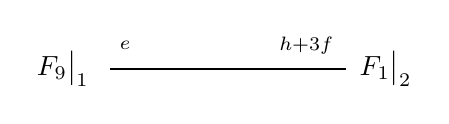
\begin{tikzpicture}
\draw[thick](-3,0)--(0,0);	
\node at(-3.6,0) {$\mathbb{F}_{9}{}\big|_1$};
\node at(-2.8,0.3) {${}_e$};
\node at(0.5,0) {$\mathbb{F}_{1}{}\big|_2$};
\node at(-0.5,0.3) {${}_{h+3f}$};
\end{tikzpicture}
\end{align}
This geometry is non-shrinkable because the volumes of  the primitive curves
\begin{align}\label{eq:SU3_8_vol}
\vol (f_1) = 2\phi_1 - \phi_2 \, , \quad
\vol (f_2) = -\phi_1 + 2\phi_2 \, , \quad
\vol (e_2) = -3\phi_1 + \phi_2 + m\ ,
\end{align}
cannot all be non-negative at the same time in the limit $m\rightarrow0$, and thus this theory cannot have a UV completion in the geometric phase \cite{Jefferson:2018irk}. However, it was pointed out in \cite{Bhardwaj:2019jtr} that this theory can be obtained from an RG flow of the UV $SU(3)_{15/2}+1{\bf F}$ theory and the UV theory is dual to the $\mathcal{N}=2$ $G_2$ gauge theory (or $G_2+1\mathbf{Adj}$). So the duality of its parent theory ensures that the $SU(3)_8$ theory has a consistent UV completion though it has no unitary geometric realization having non-trivial Coulomb branch in the UV limit.

We will now compute the BPS spectrum of this theory by solving blowup equations in the geometric (and also gauge theory) phase and show that this theory has a unitary phase with non-trivial Coulomb branch which can be directly connected to the UV fixed point. The effective prepotential is given by
\begin{align}
\mathcal{E} &= \frac{1}{\epsilon_1 \epsilon_2} \qty(\mathcal{F} - \frac{\epsilon_1^2 + \epsilon_2^2}{12}(\phi_1 + \phi_2) + \epsilon_+^2 (\phi_1 + \phi_2)) \, , \nonumber \\
6\mathcal{F} &= 8\phi_1^3 + 21\phi_1^2 \phi_2 - 27\phi_1 \phi_2^2 + 8\phi_2^3 + 6m (\phi_1^2 - \phi_1 \phi_2 + \phi_2^2) \ .
\end{align}
We find a set of consistent magnetic fluxes given by
\begin{align}
n_1 \in \mathbb{Z} + 1/3 \, , \quad
n_2 \in \mathbb{Z} + 2/3 \, , \quad
B_{m} = -1/6 \ .
\end{align}
This set can be used to formulate a unity blowup equation. The solution to the blowup equation is listed in Table~\ref{table:SU(3)_8}. Here, we have fixed $N^{(1,1,0)}_{0,0}$ using the RG flow from the spectrum of the $SU(3)_{15/2}+1{\bf F}$ theory since it remains undetermined until $e^{-3m}$ order, though it will possibly be fixed in higher order computations. All other states are fixed by solving the blowup equation and the result is consistent with the expected RG flow from the spectrum of the  parent theories, the $SU(3)_{15/2}+1{\bf F}$ theory and the $\mathcal{N}=2$ $G_2$ theory.

\begin{table}
	\centering
	\begin{tabular}{|c|C{28ex}||c|C{28ex}|} \hline
		$ \mathbf{d} $ & $ \oplus N_{j_l, j_r}^{\mathbf{d}} (j_l, j_r) $ & $ \mathbf{d}$ & $\oplus N_{j_l, j_r}^{\mathbf{d}} (j_l, j_r) $ \\ \hline
		$ (1, 0, 0) $ & $ (0, 0) $ & $ (1, 0, 1) $ & $ (0, 1) $ \\ \hline
		$ (1, 0, 2) $ & $ (0, 2) $ & $ (1, 0, 3) $ & $ (0, 3) $ \\ \hline
		$(1, 1, 0)$ & $(0, 0)$ & $(1, 1, 1)$ & $(0, 0) \oplus (0, 1)$ \\ \hline
		$(1, 1, 2)$ & $(0, 1) \oplus (0, 2)$ & $ (1, 1, 3) $ & $ (0, 2) \oplus (0, 3) $ \\ \hline
		$(1, 2, 0)$ & $(0, 0)$ & $(1, 2, 1)$ & $(0, 0) \oplus (0, 1)$ \\ \hline
		$(1, 2, 2)$ & $(0, 0) \oplus (0, 1) \oplus (0, 2)$ & $ (1, 2, 3) $ & $ (0, 1) \oplus (0, 2) \oplus (0, 3) $ \\ \hline
		$ (1, 3, 0) $ & $ (0, 0) $ & $ (1, 3, 1) $ & $ (0, 0) \oplus (0, 1) $ \\ \hline
		$ (1, 3, 2) $ & $ (0, 0) \oplus (0, 1) \oplus (0, 2) $ & $ (1, 3, 3) $ & $ (0, 0) \oplus (0, 1) \oplus (0, 2) \oplus (0, 3) $ \\ \hline
		$(2, 0, 2)$ & $(0, \frac{5}{2})$ & $ (2, 0, 3) $ & $ (0, \frac{5}{2}) \oplus (0, \frac{7}{2}) \oplus (\frac{1}{2}, 4) $ \\ \hline
		$(2, 1, 2)$ & $(0, \frac{3}{2}) \oplus (0, \frac{5}{2})$ & $ (2, 1, 3) $ & $ (0, \frac{3}{2}) \oplus 3(0, \frac{5}{2}) \oplus 2(0, \frac{7}{2}) \oplus (\frac{1}{2}, 3) \oplus (\frac{1}{2}, 4) $ \\ \hline
		$(2, 2, 1)$ & $(0, \frac{1}{2})$ & $(2, 2, 2)$ & $(0, \frac{1}{2}) \oplus 2(0, \frac{3}{2}) \oplus (0, \frac{5}{2})$ \\ \hline
		$ (2, 2, 3) $ & $ (0, \frac{1}{2}) \oplus 3(0, \frac{3}{2}) \oplus 5(0, \frac{5}{2}) \oplus 2(0, \frac{7}{2}) \oplus (\frac{1}{2}, 2) \oplus (\frac{1}{2}, 3) \oplus (\frac{1}{2}, 4) $ & $ (2, 3, 1) $ & $ 2(0, \frac{1}{2}) \oplus (\frac{1}{2}, 0) $ \\ \hline
		$ (2, 3, 2) $ & $ 3(0, \frac{1}{2}) \oplus 3(0, \frac{3}{2}) \oplus (0, \frac{5}{2}) \oplus (\frac{1}{2}, 1) $ & $ (2, 3, 3) $ & $ 3(0, \frac{1}{2}) \oplus 6(0, \frac{3}{2}) \oplus 6(0, \frac{5}{2}) \oplus 2(0, \frac{7}{2}) \oplus (\frac{1}{2}, 1) \oplus 2(\frac{1}{2}, 2) \oplus (\frac{1}{2}, 3) \oplus (\frac{1}{2}, 4) $ \\ \hline
	\end{tabular}
	\caption{BPS spectrum of $SU(3)_8$ for $d_1 \leq 2$ and $ d_2, d_3 \leq 3 $. Here, $\mathbf{d} = (d_1, d_2, d_3)$ labels the state wrapping curve $d_1 e_2 + d_2 f_1 + d_3 f_2$.} \label{table:SU(3)_8}
\end{table}

From the BPS spectrum, one finds that three hypermultiplets with degree $(1,0,0)$, $(1,1,0)$ and $ (1, 2, 0) $ have negative masses, in the limit $m\rightarrow0$, when we take masses of all other BPS states to be non-negative. This implies that once we flop these three hypermultiplets, we can attain a unitary chamber where all BPS states including the three flopped hypermultiplets have non-negative masses. This suggests that the $SU(3)_8$ theory actually has a consistent UV fixed point, and the unitary chamber we obtained by flop transitions describes the Coulomb branch of the moduli space of the CFT fixed point (without mass deformations). Thus, our computation of the BPS spectrum strongly supports the existence of the UV completion for the $SU(3)_8$ theory.
